% =====================================================================
%  TERM PAPER -- SUBMISSION 1 of 4
%  Modern Processor Microarchitecture: Pipelining, Memory Hierarchy,
%  and Compiler Co-Design
%
%  Course : Computer Architecture
%  Instr. : Prof. Smruti R. Sarangi
%  Date   : 24 August 2026
%
%  This file is FULLY SELF-CONTAINED: it uses no external files, no
%  images, and no \include/\input.  Every figure is drawn
%  programmatically in TikZ / CircuiTikZ / pgfplots, as required.
%  Compile with pdfLaTeX (run twice so that the table of contents,
%  cross-references and the list of figures/tables settle).
% =====================================================================
\documentclass[12pt,a4paper]{report}

% ---------------------------------------------------------------------
% PAGE GEOMETRY: A4, 1in margins on ALL sides (per the Q1 LaTeX upload
% instructions). No extra binding gutter is specified there, so the
% earlier 0.5in left gutter from the MS form is removed to match.
% ---------------------------------------------------------------------
\usepackage[a4paper,left=1in,right=1in,top=1in,bottom=1in,headheight=14pt]{geometry}

\usepackage[utf8]{inputenc}
\usepackage[T1]{fontenc}
% \usepackage{lmodern}   % <-- UNCOMMENT THIS LINE ON OVERLEAF (vector fonts)
\usepackage{amsmath,amssymb,amsthm}
\usepackage{graphicx}
\usepackage{tikz}
\usepackage{circuitikz}
\usepackage{pgfplots}
\pgfplotsset{compat=1.18}
\usetikzlibrary{arrows.meta,positioning,shapes,shapes.geometric,
                decorations.pathreplacing,calc,fit,backgrounds}
\usepackage{booktabs}
\usepackage{array}
% Ragged-right paragraph column: avoids the stretched inter-word spacing
% (under/overfull boxes) that justified narrow table columns produce.
\newcolumntype{L}[1]{>{\raggedright\arraybackslash}p{#1}}
\usepackage{longtable}
\usepackage{enumitem}
\usepackage{xcolor}
\usepackage{colortbl}
\usepackage[hypcap=false]{caption}
\usepackage[skins,breakable]{tcolorbox}
\usepackage{fancyhdr}
\usepackage{titlesec}
\usepackage{tocloft}
\usepackage{listings}
\usepackage[colorlinks=true,linkcolor=blue!50!black,citecolor=blue!50!black,urlcolor=blue!50!black]{hyperref}
\usepackage{cleveref}
\usepackage{imakeidx}
\makeindex[columns=2,columnseprule=true,intoc,title=Index]
\usepackage[acronym, toc, nonumberlist]{glossaries}
\makeglossaries
\setglossarystyle{long}

% ---------------------------------------------------------------------
% Listings style used for all assembly/pseudocode snippets in this
% paper, per the requirement that code be typeset with the listings
% (or minted) package rather than as plain verbatim/typewriter text.
% ---------------------------------------------------------------------
\lstdefinelanguage{SimpleRisc}{
  morekeywords={add,sub,mul,div,and,or,not,cmp,mov,ld,st,beq,bgt,bal,call,ret,addi,subi,nop},
  sensitive=false,
  morecomment=[l]{;}
}
\lstset{
  language=SimpleRisc,
  basicstyle=\ttfamily\small,
  keywordstyle=\color{archblue}\bfseries,
  commentstyle=\color{archgray}\itshape,
  numbers=left,
  numberstyle=\tiny\color{archgray},
  numbersep=8pt,
  frame=single,
  rulecolor=\color{archgray!60},
  backgroundcolor=\color{gray!5},
  breaklines=true,
  columns=flexible,
  xleftmargin=1.2em,
  framexleftmargin=1em,
  captionpos=b
}

% ---------------------------------------------------------------------
% SINGLE-SPACING (explicit, since the default is already single-spaced
% in the report class -- kept here as a documented, deliberate choice
% rather than an accident of the class defaults).
% ---------------------------------------------------------------------
\renewcommand{\baselinestretch}{1.0}

% A little extra stretch so long technical words never force an overfull
% line; keeps the log clean without resorting to \sloppy everywhere.
\setlength{\emergencystretch}{3em}

% Float-only pages align to the top rather than being vertically centred.
\makeatletter
\setlength{\@fptop}{0pt}
\makeatother

% Table of contents shows chapters, sections and subsections.
\setcounter{tocdepth}{2}

% ---------------------------------------------------------------------
% Headers/footers
% ---------------------------------------------------------------------
\pagestyle{fancy}
\fancyhf{}
\fancyhead[R]{\thepage}
\fancyhead[L]{\nouppercase{\leftmark}}
\renewcommand{\headrulewidth}{0.4pt}

% ---------------------------------------------------------------------
% TikZ / circuitikz color palette tied to the theme, so every diagram
% in the paper looks consistent regardless of who draws it.
% ---------------------------------------------------------------------
\definecolor{archblue}{RGB}{31,78,121}
\definecolor{archorange}{RGB}{198,120,40}
\definecolor{archgray}{RGB}{110,110,110}
\definecolor{archgreen}{RGB}{40,120,80}

% Reusable style for "pipeline diagram" grid figures (stage x cycle grids
% showing which instruction occupies which stage in which cycle).
\tikzset{
  pdbox/.style={draw, thick, minimum width=0.85cm, minimum height=0.72cm,
    font=\footnotesize, align=center},
  pdlabel/.style={font=\footnotesize\bfseries, archgray},
  pdarrow/.style={-{Stealth[length=2mm]}, thick, archorange}
}

% Block styles used by the schematic figures of Chapter 2.
\tikzset{
  box/.style={draw, rounded corners, minimum height=0.9cm, minimum width=2.1cm,
              align=center, font=\small, fill=gray!8},
  smallbox/.style={draw, minimum height=0.8cm, minimum width=1.4cm,
              align=center, font=\footnotesize},
  arr/.style={-{Latex[length=2mm]}, thick}
}

% ---------------------------------------------------------------------
% FORWARD REFERENCES TO CHAPTERS AND PARTS NOT YET WRITTEN.
%
% Chapter 1 refers, by design, to chapters and parts that will only be
% written in submissions 2--4.  So that \cref/\ref still typeset the
% correct, intended numbers in this draft (instead of "??"), we reserve
% those numbers here with two dedicated counters.  The reservations are
% all declared, invisibly, at the start of Appendix E, next to the table
% that lists the planned chapters.  Nothing is printed by these macros.
% ---------------------------------------------------------------------
\newcounter{planch}
\newcounter{planpt}
\renewcommand{\theplanch}{\arabic{planch}}
\renewcommand{\theplanpt}{\Roman{planpt}}
\crefname{planch}{chapter}{chapters}
\Crefname{planch}{Chapter}{Chapters}
\crefname{planpt}{part}{parts}
\Crefname{planpt}{Part}{Parts}
% Spell "figure" out rather than using cleveref's default "fig.", so that
% figure, table and section references read consistently.
\crefname{figure}{figure}{figures}
\Crefname{figure}{Figure}{Figures}
\newcommand{\planchlabel}[2]{%
  \setcounter{planch}{#2}\addtocounter{planch}{-1}%
  \refstepcounter{planch}\label{#1}\ignorespaces}
\newcommand{\planptlabel}[2]{%
  \setcounter{planpt}{#2}\addtocounter{planpt}{-1}%
  \refstepcounter{planpt}\label{#1}\ignorespaces}

% ---------------------------------------------------------------------
% A framed box used only in Appendix E, to mark the space deliberately
% left open for the team's own additions to the forward plan.
% ---------------------------------------------------------------------
\definecolor{plannedbg}{RGB}{245,245,250}
\definecolor{plannedbar}{RGB}{90,90,160}
\newtcolorbox{openspace}[1][]{%
  breakable, enhanced,
  colback=plannedbg, colframe=plannedbar,
  boxrule=0pt, leftrule=2.5pt,
  arc=0pt, outer arc=0pt,
  left=8pt, right=8pt, top=6pt, bottom=6pt,
  before skip=8pt, after skip=8pt,
  fonttitle=\bfseries\small, #1}

% ---------------------------------------------------------------------
% Gantt-chart drawing macros (Appendix D).  Everything is plain TikZ --
% no external Gantt package -- so the file stays self-contained and the
% figure stays compliant with the "figures must be drawn in TikZ" rule.
%
%   \wpheader{row}{text}          -- a work-package banner row
%   \gtask{row}{start}{end}{frac}{label}
%                                 -- one task bar; "frac" in [0,1] is the
%                                    fraction complete, drawn as a solid
%                                    overlay on a hollow planned bar.
% One horizontal unit = one calendar week.
% ---------------------------------------------------------------------
\newcommand{\ganttleft}{-12.6}
\newcommand{\wpheader}[2]{%
  \fill[archblue!18] (\ganttleft,-#1-0.34) rectangle (14,-#1+0.34);
  \node[anchor=west, font=\scriptsize\bfseries, archblue]
    at ({\ganttleft+0.1},-#1) {#2};}
\newcommand{\gtask}[5]{%
  \node[anchor=west, font=\scriptsize] at ({\ganttleft+0.3},-#1) {#5};
  \draw[archgray!55, fill=archblue!12] (#2,-#1-0.26) rectangle (#3,-#1+0.26);
  \ifdim #4pt>0pt
    \fill[archblue!75] (#2,-#1-0.26) rectangle ({#2+(#3-#2)*#4},-#1+0.26);
  \fi}

% ---------------------------------------------------------------------
% Glossary entries. Terms actually developed in the written chapters of
% this draft; \gls{} is used at first mention in the body text below,
% and \printglossary (with \glsaddall) lists every entry regardless of
% how many times each is actually referenced. Descriptions are kept to
% one line each so the printed glossary (table style, no letter
% grouping) fits on a single page.
% ---------------------------------------------------------------------
\newglossaryentry{hazard}{name={Hazard},
  description={Risk of an incorrect result because an instruction's inputs are not yet ready}}
\newglossaryentry{rawhazard}{name={RAW hazard},
  description={A later instruction reads a value before an earlier one has written it}}
\newglossaryentry{forwarding}{name={Forwarding},
  description={Routes a value directly between pipeline stages, bypassing the register file}}
\newglossaryentry{structuralhazard}{name={Structural hazard},
  description={Two instructions needing the same hardware resource in the same cycle}}
\newglossaryentry{controlhazard}{name={Control hazard},
  description={Risk of fetching the wrong instruction because a branch is not yet resolved}}
\newglossaryentry{loaduse}{name={Load-use hazard},
  description={The one RAW hazard forwarding cannot fix; costs exactly one stall cycle}}
\newglossaryentry{isa}{name={Instruction set architecture},
  description={The operations and encodings through which software makes use of hardware}}
\newglossaryentry{pipelining}{name={Pipelining},
  description={Overlapping multiple instructions across pipeline stages to raise throughput}}
\newglossaryentry{amat}{name={AMAT},
  description={Average memory access time: hit time plus miss rate times miss penalty}}
\newglossaryentry{memorywall}{name={Memory wall},
  description={The widening gap between processor speed and main memory speed}}
\newglossaryentry{workingset}{name={Working set},
  description={The slowly changing subset of memory a program mostly references}}
\newglossaryentry{dennard}{name={Dennard scaling},
  description={Trend of smaller transistors also being faster and lower-power; ended mid-2000s}}
\newglossaryentry{delayedbranch}{name={Delayed branch},
  description={Filling branch-delay slots with useful, branch-independent instructions}}
\newglossaryentry{bubble}{name={Pipeline bubble},
  description={An inert no-op inserted into a stage in place of a stalled instruction}}
\newglossaryentry{interlock}{name={Hardware interlock},
  description={Stall mechanism that detects a hazard and freezes the pipeline to stay correct}}
\newglossaryentry{throughput}{name={Throughput},
  description={Rate of instruction completion, as distinct from any single instruction's latency}}
\newglossaryentry{cpi}{name={CPI},
  description={Cycles per instruction: average clock cycles spent per instruction executed}}
\newglossaryentry{risc}{name={RISC},
  description={ISA philosophy favouring simple, uniform, fixed-latency instructions}}
\newglossaryentry{simplerisc}{name={SimpleRISC},
  description={The load-store instruction set used for derivations throughout this paper}}
\newglossaryentry{branchprediction}{name={Branch prediction},
  description={Hardware guess of a branch's direction and target before it is evaluated}}
\newglossaryentry{superscalar}{name={Superscalar},
  description={Fetching and executing more than one instruction per cycle}}
\newglossaryentry{oooexec}{name={Out-of-order execution},
  description={Instructions may complete out of program order if dependences are respected}}
\newglossaryentry{regalloc}{name={Register allocation},
  description={Assigning a program's values to a finite set of physical registers}}
\newglossaryentry{vliw}{name={VLIW},
  description={Compiler packs multiple operations into one wide instruction at compile time}}
\newglossaryentry{branchpenalty}{name={Branch penalty},
  description={Cycles wasted per mispredicted (or, conservatively, every) branch}}

\title{\textbf{Modern Processor Microarchitecture:\\[4pt]
\Large Pipelining, Memory Hierarchy, and\\ Compiler Co-Design}\\[10pt]
\large A study of how instruction execution, the memory system, and the\\
compiler jointly determine processor performance}
\author{
\textit{Author 1 Arnab Mandal} \quad \textit{2024EE10454} \\
\textit{Author 2 Saksham Kumar} \quad \textit{2024EE10044} \\
\textit{Author 3 Keshav Kumar Ramuka} \quad \textit{2024EE10363} \\[8pt]
\href{https://github.com/arnabmandal-5090/Computer-Architecture-Term-Paper---Modern-Processor-Microarchitecture/new/main}{GitHub Repository}
\quad\textbar\quad
\href{https://www.zotero.org/groups/6645711/term_paper_references_67}{Zotero Group Library}
}

\date{
\textbf{ELL305: Computer Architecture}\\
Instructor: Prof. Sumantra Dutta Roy and Prof. Subrat Kar\\[6pt]
Submission 1 of 4 \textbf{--- 24 August 2026}
}

\begin{document}

\maketitle

\newpage
\thispagestyle{empty}
\vspace*{2cm}
\begin{center}
{\Large\bfseries Copyright Assignment}
\end{center}
\vspace{1.5cm}
\noindent
All intellectual property rights (IPR) in this term paper, including its
text, figures, diagrams, and derivations, belong to the Indian Institute
of Technology Delhi (IIT Delhi), except where material has been cited
from an external source, in which case intellectual property rights in
that cited material remain with the respective authors of the original
source. Every such source is credited at its point of use and listed in
full in the Bibliography.

\newpage
\thispagestyle{empty}
\vspace*{2cm}
\begin{center}
{\Large\bfseries Acknowledgements}
\end{center}
\vspace{1.5cm}
\noindent
We are grateful to Prof.\ Sumantra Dutta Roy and Prof.\ Subrat Kar for
their guidance throughout the development of this term paper, and to
our peers in ELL305 for helpful discussion during its drafting. We
gratefully acknowledge the Department of Electrical Engineering, IIT
Delhi, for the computing resources, library access, and academic
environment that made this work possible, and IIT Delhi more broadly
for the infrastructure, including Gradescope and institutional access
to the cited literature, that supported this submission.

\newpage

\begin{abstract}
\noindent
A processor's execution resources, its memory system, and the compiler
that targets it are conventionally taught as three separate subjects,
each with its own chapter, its own vocabulary, and its own body of
technique. This paper takes the position that they are better understood
as three views of a single underlying problem: how to keep a fast
execution pipeline supplied with correct data at the right moment, given
that main memory is several hundred times slower than the processor
consuming it, and that the hardware alone cannot always see far enough
ahead to plan around that gap. We develop this argument across three
parts, moving from hardware toward software rather than treating the
three domains as parallel, unconnected tracks.

The first part derives how a classical five-stage pipeline sustains
close to one instruction per cycle in the presence of data, control, and
structural hazards, then extends this into the territory where static,
in-order execution stops being sufficient: dynamic branch prediction\index{branch prediction}\glsadd{branchprediction},
superscalar\index{superscalar}\glsadd{superscalar} issue, and out-of-order completion\index{out-of-order execution}\glsadd{oooexec}. The second part asks why
no single memory technology can be simultaneously fast, large, and
inexpensive, derives that coupling from the circuit-level behaviour of
SRAM and DRAM cells, and shows how a multi-level hierarchy of caches,
address translation, and cross-core coherence turns a several-hundred-cycle
DRAM access into an average latency close to that of the fastest level
in the hierarchy. The third part turns to the compiler, showing how
instruction scheduling and register allocation\index{register allocation}\glsadd{regalloc} let software absorb
decisions at compile time that the first two parts would otherwise have
to pay for at run time, and contrasts this compile-time philosophy
directly against the VLIW\index{VLIW}\glsadd{vliw} and EPIC attempt to remove hardware's role in
scheduling altogether.

Two commitments run through all three parts. First, every mechanism is
derived rather than merely described: hazards are shown to force
forwarding and stalling, the physics of memory cells is shown to force
a hierarchy, and a compiler's visibility into a program is shown to
force particular scheduling choices, rather than simply asserting that
this is how it is done. Second, real, currently shipping processors,
among them AMD's Zen line, Intel's Golden Cove and Lion Cove cores, and
Apple's M-series chips, are used throughout as worked evidence that the
theory actually describes hardware people use today, not only as
decoration. A closing chapter ties the three parts together by tracing a
single small benchmark through all three mechanisms on two real
architectures, and, where measurement is feasible, compares the
theoretical predictions of the earlier chapters against what real
hardware performance counters actually report. Every diagram in this
paper, including pipeline timing diagrams, cache organisation figures,
and coherence-protocol state machines, is produced programmatically in
TikZ or CircuiTikZ rather than imported as an image.

Taken together, these three perspectives show that processor
performance is not determined by execution units, memory technology, or
compiler decisions in isolation. It emerges from the interaction
between them, with each layer compensating for limitations that remain
at the others. The paper treats modern computer architecture
as a coordinated hardware--software system whose performance depends on
how effectively these layers work together.
\end{abstract}


\tableofcontents
\listoffigures
\listoftables

\renewcommand*{\descriptionname}{Explanation}
\renewcommand{\glossarypreamble}{%
  \noindent Terms are drawn from their first use in \cref{ch:intro,ch:pipeline-basics}.\par}
\glsaddall
\begingroup
\footnotesize
\renewcommand{\arraystretch}{0.85}
\setlength{\glsdescwidth}{0.74\textwidth}
\printglossary[title={Glossary},nopostdot,nonumberlist]
\endgroup

% =======================================================================
\chapter{Introduction}
\label{ch:intro}

\section{The Central Problem}
\label{sec:central-problem}

Consider a processor designed with real care. It fetches, decodes, and
issues four instructions per cycle. Its branch predictor is correct
nineteen times in twenty. Its execution units are fully pipelined and
never themselves stall. In isolation, every one of its components is
excellent, and a designer evaluating them individually would have every
reason for confidence. Connect this processor to a realistic memory
system and a realistic instruction stream, however, and its measured
throughput falls to a fraction of its four-wide potential. Two effects,
independent of each other and independent of anything wrong with the
execution units themselves, are responsible.

The first is the branch predictor's one failure in twenty. Modern
pipelines are deep enough that a misprediction is not discovered until
several stages after the branch was fetched, so recovering from it means
discarding a substantial amount of speculative work and restarting fetch
from the correct address. The second effect, and generally the larger
one, is memory. A load that misses the entire on-chip cache hierarchy
and must be serviced by DRAM stalls its dependents for on the order of
two hundred cycles. That is long enough for the four-wide core to have
completed several hundred arithmetic operations, had it had something
else to do in the meantime.

It is possible to quantify which of these two effects matters more, and
the arithmetic is worth doing before either mechanism is studied in
detail, because it decides how much of this paper's effort belongs to
each. Model the stall contribution of each effect as a rate of
occurrence multiplied by a penalty:
\begin{align}
\text{Stall cycles per instruction (memory)} &= f_{\text{mem}} \cdot m_{\text{global}} \cdot t_{\text{DRAM}}, \label{eq:mem-stall} \\
\text{Stall cycles per instruction (branch)} &= f_{\text{branch}} \cdot p_{\text{mispredict}} \cdot t_{\text{flush}}. \label{eq:branch-stall}
\end{align}
Take representative figures for a general-purpose workload. Roughly 30\%
of instructions access memory ($f_{\text{mem}} = 0.30$), of which
perhaps 2\% miss all the way to DRAM after filtering through the cache
hierarchy ($m_{\text{global}} = 0.02$), at a DRAM penalty of
$t_{\text{DRAM}} = 200$ cycles. For branches, take a frequency of one in
five instructions ($f_{\text{branch}} = 0.20$), a predictor accuracy in
line with the 95\% figure above ($p_{\text{mispredict}} = 0.05$), and a
moderate pipeline flush penalty of $t_{\text{flush}} = 15$ cycles.
Substituting into \cref{eq:mem-stall,eq:branch-stall}:
\[
0.30 \times 0.02 \times 200 = 1.2 \text{ cycles/instr.}
\qquad\text{versus}\qquad
0.20 \times 0.05 \times 15 = 0.15 \text{ cycles/instr.}
\]
Under these representative numbers, memory stalls cost roughly eight
times what branch mispredictions cost, despite memory being the
\emph{rarer} of the two failure modes by an order of magnitude
($m_{\text{global}} = 0.02$ against $p_{\text{mispredict}} = 0.05$). The
reason is that the memory penalty is itself more than an order of
magnitude larger than the branch penalty\index{branch penalty}\glsadd{branchpenalty}. This is the arithmetic
signature that recurs throughout computer architecture: rare, expensive
events dominate common, cheap ones. It is the reason \cref{part:memory}
of this paper is proportionally the largest of the three technical
parts.

The comparison also explains why the other two pillars remain necessary
rather than optional. First, $t_{\text{flush}}$ in \cref{eq:branch-stall}
is not a fixed constant. It grows with pipeline depth and issue width,
so a wider, deeper core built to reduce $\text{CPI}_{\text{base}}$
mechanically makes branch mispredictions more expensive, even as it
makes memory stalls relatively more dominant still, a point we return to
formally once \cref{ch:memcells} develops the \gls{amat}\index{AMAT (average memory access time)} model. Studying
pipelining and branch prediction (\cref{part:pipeline}) is thus
inseparable from studying why memory matters as much as it does. Second,
neither $m_{\text{global}}$ nor the hazard stalls absorbed silently
inside $\text{CPI}_{\text{base}}$ are fixed by the hardware alone. A
compiler that schedules instructions and unrolls loops well changes both
terms before the program ever runs, which is the subject of
\cref{part:compiler}. The three parts of this paper are not three
independent topics that happen to share a course. They are three levers
on the same two equations. The particular historical circumstances that
made this trio unavoidable together, namely the end of Dennard scaling
and the industry's shift to multicore designs, are a substantial enough
digression that they are developed separately in
\cref{app:history-trio} rather than here.

\section{Why Each Piece Is Hard}
\label{sec:why-hard}

\subsection{The Pipeline's Correctness Problem}
Executing instructions one after another in a pipeline is only free if
each instruction's inputs are ready when the pipeline reaches the stage
that needs them, and if the identity of the next instruction to fetch is
already known. Neither is guaranteed. An instruction may need the result
of one still in flight (a data hazard\index{hazard!data}), two instructions may need the
same hardware resource in the same cycle (a structural hazard\index{hazard!structural}\glsadd{structuralhazard}), and a
branch's outcome and target are, by construction, not known until the
branch itself has been evaluated (a control hazard\index{hazard!control}\glsadd{controlhazard}).
\Cref{ch:pipeline-basics} develops each of these precisely and derives
the hardware and software mechanisms, among them forwarding, stalling,
and prediction, that resolve them without giving up the pipeline's
throughput. This difficulty predates the five-stage pipeline studied in
this paper by several decades; its pedigree, running from Tomasulo's
algorithm through the reduced-instruction-set philosophy, is traced in
\cref{app:history-pillars}.

\subsection{The Coupling Between Latency, Capacity, and Cost}
A memory built entirely from the fastest available technology, sized to
hold everything a program touches, would remove the two-hundred-cycle
penalty in \cref{eq:mem-stall} entirely. It cannot be built, because
access latency, storage capacity, and cost per bit are coupled by
physics (wire delay and cell area both scale with array size) and by
economics (the cell designs that are fast are not the cell designs that
are dense), in a way that no single technology has ever escaped.
\Cref{ch:memcells,ch:caches} derive this coupling from circuit-level
first principles and show how a layered hierarchy is the direct, forced
consequence of it. The empirical shape of this problem, established
well before the transistor budgets of modern chips made it as severe as
it now is, is traced back to Denning, Mattson, and Wulf and McKee in
\cref{app:history-pillars}.

\subsection{The Compile-Time and Run-Time Information Gap}
A compiler can see the entire structure of a loop, every dependence and
every iteration, before the program ever runs. A processor sees only a
narrow, moving window of in-flight instructions. This asymmetry means
some scheduling decisions are cheaper to make once, at compile time
(instruction ordering, register allocation), while others are
fundamentally impossible to make until run time, such as whether a
particular load will hit or miss the cache.
\Cref{ch:compiler-sched,ch:regalloc,ch:ilp-philosophy} study how far
compile-time scheduling can be pushed, and \cref{ch:ilp-philosophy} in
particular studies what happens, under the VLIW and EPIC design
philosophy, when an architecture tries to push it all the way. This gap
is not merely theoretical; Fisher's ELI-512 work, which first
demonstrated it concretely, is discussed in \cref{app:history-pillars}.

\section{Aims of This Paper}
\label{sec:aims}

Given the problem above, this paper aims to:
\begin{enumerate}[leftmargin=*]
  \item derive, rather than assert, why pipelining alone is insufficient
    without explicit hazard handling and branch prediction, and develop
    the hardware mechanisms (forwarding, dynamic prediction, and
    out-of-order issue) that address this (\cref{part:pipeline});
  \item derive, rather than assert, why a single level of memory cannot
    be simultaneously fast, large and cheap, and show quantitatively how
    a multi-level hierarchy resolves this, extending the argument to
    multicore coherence and consistency (\cref{part:memory});
  \item show how a compiler's static scheduling decisions, among them
    loop unrolling, software pipelining, and register allocation, reduce
    the burden placed on the hardware mechanisms of \cref{part:pipeline},
    and contrast this compile-time approach with the run-time approach of
    out-of-order execution (\cref{part:compiler});
  \item connect all three mechanisms to real, shipping designs (AMD's
    Zen microarchitecture, Intel's Golden/Lion Cove cores, Apple's
    M-series, and ARM's Cortex family) as worked case studies that
    validate the theory developed, rather than as the paper's primary
    content; and
  \item close with a single synthesis chapter (\cref{ch:synthesis}) that
    traces one small benchmark through all three mechanisms on two real
    architectures, so that the three parts are shown operating as one
    system rather than as three independent topics; and
  \item where feasible given the time and hardware access available to a
    three-person team, go beyond exposition in \cref{ch:synthesis} by
    \emph{measuring} real hardware performance counters for the chosen
    benchmark and testing whether the theoretical models developed in
    \cref{part:pipeline,part:memory} actually predict what is measured.
    This is an empirical question the paper does not know the answer to
    in advance, rather than a description of a known result.
\end{enumerate}

\section{Non-Aims}
\label{sec:non-aims}

Several adjacent and legitimate topics are deliberately excluded, in
order to treat the material above in depth rather than treat a wider
syllabus shallowly. We do not treat GPU architecture as a full pillar;
it appears only briefly, as a contrasting case study in
\cref{ch:coherence}, where the unified memory model of Apple's M-series
is compared against discrete CPU/GPU memory systems. We do not treat
operating-system internals beyond the page-replacement policies that
virtual memory requires, and we do not treat process scheduling,
file systems, or I/O subsystems at all. We do not treat SIMD/vector
ISA extensions in detail, beyond noting where they interact with the
memory system. Circuit-level material in \cref{ch:memcells} is developed
only to the depth needed to establish the architectural consequence that
follows from it (the necessity of a hierarchy); a rigorous treatment of
CMOS device physics is outside this paper's scope and is available in
standard VLSI texts. Finally, this paper studies compiler
\emph{scheduling} decisions as they interact with the microarchitecture
(\cref{part:compiler}); it does not treat compiler front-end topics such
as parsing, type systems, or source-level optimization that have no
direct architectural consequence.



\begin{table}[htbp]
\centering
\caption{Mapping between the chapters of this paper and the prescribed
textbook, Sarangi, \emph{Basic Computer Architecture}. Page numbers refer
to the edition used in this course. Where the prescribed text does not
cover a chapter's material, the primary external source is given instead.}
\label{tab:textbook-map}
\begin{tabular}{@{}L{0.40\textwidth}L{0.52\textwidth}@{}}
\toprule
\textbf{This paper} & \textbf{Sarangi, \emph{Basic Computer Architecture}} \\
\midrule
Ch.~\ref{ch:pipeline-basics}: Pipeline Fundamentals \& Hazards &
  Ch.~10 \emph{Principles of Pipelining}, \S10.1--\S10.6 (pp.~413--457):
  the pipelined datapath, pipeline stages, and structural/data/control
  hazards, including software (interlock) and hardware (forwarding)
  solutions. \\
Ch.~\ref{ch:branch-ooo}: Branch Prediction \& Out-of-Order Execution &
  Ch.~10, \S10.9 \emph{Advanced Techniques} (pp.~487--497): branch
  prediction, multiple-issue in-order pipelines, EPIC/VLIW processors,
  and out-of-order pipelines. \\
Ch.~\ref{ch:memcells}: Memory Cells and the Case for a Hierarchy &
  Ch.~9 \emph{Logic Gates, Registers, and Memories}, \S9.4 \emph{Memories}
  (pp.~288--297: SRAM, CAM, DRAM, ROM); Ch.~11 \emph{The Memory System},
  \S11.1 \emph{Overview} (pp.~508--518). \\
Ch.~\ref{ch:caches}: Cache Organisation and Optimisation &
  Ch.~11, \S11.2 \emph{Caches} and \S11.3 \emph{The Memory System}
  (pp.~519--541): cache lookup and design, the mathematical model of the
  memory system, and miss classification. \\
Ch.~\ref{ch:coherence}: Multicore Memory: Coherence, Consistency \&
  Prefetching &
  Ch.~11, \S11.4 \emph{Virtual Memory} (pp.~541--560); Ch.~12
  \emph{Multiprocessor Systems}, \S12.4 \emph{Coherence} and
  \S12.4 \emph{Memory Consistency} (pp.~583--610). \\
Ch.~\ref{ch:compiler-sched}: Static Scheduling \& Loop Transformations &
  Ch.~10, \S10.7 \emph{Inter-Relationship between Performance, the
  Compiler, Architecture, and Technology} (p.~476), extended primarily
  from \cite{shen}, Ch.~2 (instruction scheduling). \\
Ch.~\ref{ch:regalloc}: Register Allocation \& Backend Code Generation &
  Not covered in the prescribed text; developed from Hennessy and
  Patterson \cite{hennessy}, Appendix~A, and standard compiler-construction
  references. \\
Ch.~\ref{ch:ilp-philosophy}: VLIW vs.\ Superscalar &
  Ch.~10, \S10.9.3 \emph{EPIC and VLIW Processors} and \S10.9.4
  \emph{Out-of-Order Pipelines} (pp.~493--497). \\
Ch.~\ref{ch:synthesis}: Synthesis Case Study &
  Appendix~A \emph{Case Studies of Real Processors} (pp.~733--753: ARM
  Cortex-M3/A8/A15, AMD Bobcat/Bulldozer, Intel Atom/Sandy Bridge) and
  Appendix~A, \S A.2 \emph{Graphics Processors} (pp.~753--762). \\
\bottomrule
\end{tabular}
\end{table}

\section{Organisation of This Paper}
\label{sec:organisation}

The paper is organised into five parts, sketched in \cref{fig:roadmap}.
\Cref{part:pipeline} (Pipelining and Instruction Execution) develops the
classical pipeline datapath and the three hazard types in
\cref{ch:pipeline-basics}, then extends this in \cref{ch:branch-ooo} to
the dynamic mechanisms, namely branch prediction, superscalar issue, and
out-of-order execution, that hardware uses when static scheduling alone
is not enough. \Cref{part:memory} (The Memory Hierarchy) begins from
circuit-level storage cells in \cref{ch:memcells}, builds the
cache-organisation and replacement machinery that sits above them in
\cref{ch:caches}, and extends the single-core picture to coherence,
consistency and prefetching across multiple cores in \cref{ch:coherence}.
\Cref{part:compiler} (Compiler--Architecture Co-Design) studies the
opposite lever: how a compiler's static scheduling
(\cref{ch:compiler-sched}) and register allocation
(\cref{ch:regalloc}) reduce the burden on the mechanisms of
\cref{part:pipeline}, closing with a direct contrast between compile-time
and run-time ILP extraction in \cref{ch:ilp-philosophy}. Finally,
\cref{part:synthesis} draws the three parts together: \cref{ch:synthesis}
traces one benchmark through all three mechanisms on two real
architectures, and \cref{ch:conclusion} closes with open problems that
span all three pillars at once, such as speculative-execution side
channels that arise precisely at the boundary between
\cref{ch:branch-ooo,ch:caches}. Chapters~1 and~2 are complete as of this
submission; the remaining chapters are outlined at the section level
below and will be completed across the subsequent draft submissions,
converging on a final paper of approximately 150 pages.

\begin{figure}[htbp]
\centering
\resizebox{\textwidth}{!}{%
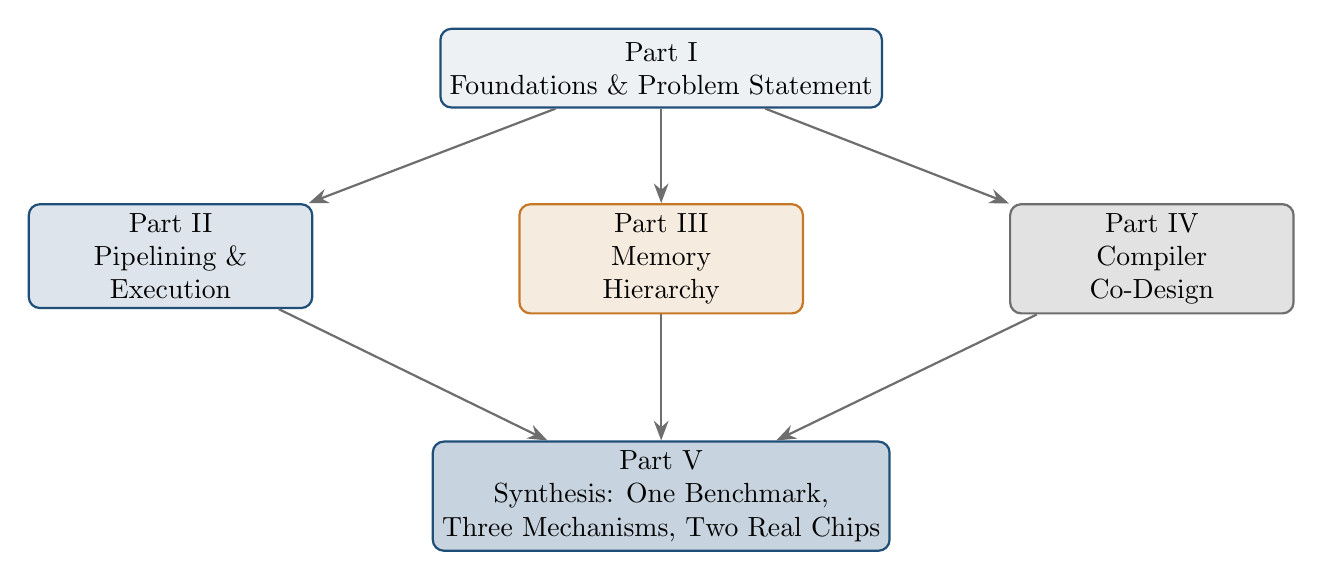
\begin{tikzpicture}[
  block/.style={draw, rounded corners, minimum width=3.6cm, minimum height=1cm,
    align=center, fill=archblue!8, draw=archblue, thick},
  pillar/.style={draw, rounded corners, minimum width=3.6cm, minimum height=1.3cm,
    align=center, thick},
  arr/.style={-{Stealth[length=2.5mm]}, thick, archgray}
]
  \node[block] (intro) {Part I\\Foundations \& Problem Statement};
  \node[pillar, fill=archblue!15, draw=archblue, below left=1.2cm and 1.6cm of intro] (pA)
    {Part II\\Pipelining \&\\Execution};
  \node[pillar, fill=archorange!15, draw=archorange, below=1.2cm of intro] (pB)
    {Part III\\Memory\\Hierarchy};
  \node[pillar, fill=archgray!20, draw=archgray, below right=1.2cm and 1.6cm of intro] (pC)
    {Part IV\\Compiler\\Co-Design};
  \node[block, below=1.6cm of pB, fill=archblue!25] (synth)
    {Part V\\Synthesis: One Benchmark,\\Three Mechanisms, Two Real Chips};

  \draw[arr] (intro) -- (pA);
  \draw[arr] (intro) -- (pB);
  \draw[arr] (intro) -- (pC);
  \draw[arr] (pA) -- (synth);
  \draw[arr] (pB) -- (synth);
  \draw[arr] (pC) -- (synth);
\end{tikzpicture}}
\caption{Roadmap of the paper. Parts~I and~II attack the problem from the
hardware side, Part~III from the compiler side, and Part~IV draws all
three together around one worked example.}
\label{fig:roadmap}
\end{figure}

\section{Notation and Conventions}
\label{sec:notation}

The following symbols are fixed for use across all three parts of this
paper, so that a reader (and each of the three authors) can move between
chapters without re-learning notation.

\begin{table}[htbp]
\centering
\caption{Notation used throughout this paper.}
\label{tab:notation}
\begin{tabular}{@{}L{0.16\textwidth}L{0.78\textwidth}@{}}
\toprule
\textbf{Symbol} & \textbf{Meaning} \\
\midrule
$B$ & Cache block (line) size, in bytes. \\
$S$ & Number of sets in a cache. \\
$W$ & Associativity (number of ways per set). \\
$C = B \cdot S \cdot W$ & Total cache capacity, in bytes. \\
$h$ & Hit rate at a given level of the hierarchy. \\
$m$ & Miss rate at a given level ($m = 1-h$); $m_{\text{local}}$ and
  $m_{\text{global}}$ are distinguished where both are used. \\
$t_{\text{hit}}$, $t_{\text{penalty}}$ & Hit time and miss penalty (additional
  latency on a miss) for a cache level, in processor cycles. \\
$\text{AMAT}$ & Average memory access time, $t_{\text{hit}} + m \cdot
  t_{\text{penalty}}$, extended recursively for multiple levels. \\
IPC, CPI\index{CPI (cycles per instruction)}\glsadd{cpi} & Instructions per cycle and cycles per instruction
  ($\text{CPI} = 1/\text{IPC}$ for a scalar pipeline; both are quoted
  for superscalar designs since they are not exact reciprocals once
  issue width $> 1$). \\
Issue width & Maximum number of instructions a core can fetch/issue in
  one cycle. \\
ROB & Reorder buffer; ROB size denotes its entry count. \\
$f_{\text{mem}}$, $f_{\text{branch}}$ & Fraction of dynamic instructions
  that are memory operations, and that are branches, respectively. \\
\bottomrule
\end{tabular}
\end{table}

Addresses are treated as $n$-bit unsigned integers, bit~0 least
significant. Capacities follow the binary convention
($1\,\text{KB} = 2^{10}$ bytes, $1\,\text{MB} = 2^{20}$ bytes). Latencies
are quoted in processor clock cycles unless a unit is given explicitly.
Assembly examples used for derivation (as opposed to case-study material
quoting a specific vendor's ISA) use the SimpleRisc\index{SimpleRISC}\glsadd{simplerisc} instruction set of
\cite{sarangi} (Ch.~3), so that they can be read without reference to any
particular commercial ISA; case-study boxes that quote real compiler
output use x86-64 or AArch64 explicitly, as noted at each occurrence.

% =======================================================================
\chapter{Instruction Set Design and Pipelining}
\label{ch:pipeline-basics}

\section{Instruction Set Design and Its Relevance to Pipelining}
\label{sec:isa-tradeoffs}

\subsection{Instruction Set Design}

The instruction set architecture (ISA)\index{instruction set architecture (ISA)}\glsadd{isa} defines the operations a processor can perform and the interface through which software makes use of those operations. At a basic level, an ISA has to be complete for the kind of programs it is intended to run: it must provide enough functionality for those programs to be expressed in machine code. What counts as sufficient functionality depends on the target workload. A general-purpose processor needs to support a broad range of programs, whereas a specialized embedded processor can afford to leave out operations that its applications do not require. ISA design is, in this sense, a matter of deciding what capabilities should be exposed to software while keeping the underlying implementation practical. Completeness, conciseness, generality, and simplicity are useful principles in making these choices.

Conciseness matters because every instruction has to be supported by hardware. As the number of instructions grows, so does the amount of decoding and control logic needed to recognize and implement them, increasing the overall complexity of the processor. It is undesirable to add specialized instructions when the same functionality can be expressed reasonably well using a smaller set of useful operations. The principle of generality leads to a similar conclusion: instructions should primarily support operations that occur frequently in programs. Common arithmetic and logical operations are good candidates for direct hardware support, while less frequently used computations can often be built from existing instructions or provided through software libraries. The ISA consequently reflects a compromise between what software needs and what the hardware can implement efficiently.

Among these properties, simplicity is especially relevant when the ISA is considered together with the processor datapath. A simple instruction, such as an addition of two operands, can be implemented through a relatively straightforward sequence of hardware operations. A more complex instruction may instead accept several operands or combine multiple forms of computation into a single operation. The simpler approach may cause the compiler to generate more instructions, but each instruction has a more regular execution structure. This distinction underlies the conventional RISC-CISC classification: RISC\index{RISC}\glsadd{risc} architectures favor simple, regular instructions, whereas CISC architectures support a larger and more varied collection of complex instructions. For a pipelined implementation, the important issue is not simply how many instructions an ISA contains, but how regular the operations are that the hardware must accommodate.~\cite{sarangi}

\subsection{ISA Regularity, Encoding, and the Datapath}

This regularity becomes important once instruction execution is divided into pipeline stages. A pipeline repeatedly applies a sequence of datapath operations to successive instructions, with different instructions occupying different stages at the same time. When instructions have relatively predictable forms and require similar categories of processing, the datapath can be divided into stages with a more consistent flow of work. Greater variation in instruction behavior, on the other hand, can require additional control and datapath functionality. The ISA, in turn, places constraints on the organization of the processor that ultimately implements it. This does not imply that a simple or RISC-style ISA automatically produces an efficient pipeline; rather, regularity gives the microarchitecture a more predictable set of operations around which the pipeline can be organized.

The connection becomes clearer when instruction encoding is considered. A regular ISA can use a small number of well-defined instruction formats, such as register, immediate, and branch formats. If the encoding is arranged so that the processor can identify the relevant format from particular instruction fields, decoding becomes a more structured part of the instruction-processing path. This matters particularly in the early stages of a pipeline, where an instruction must be fetched, interpreted, and prepared for the work that follows without adding unnecessary complexity to the critical path.

The same idea extends to operands and addressing modes. An instruction may obtain an operand directly from a register, use an immediate value, or require an effective address to be calculated before accessing memory. These architectural choices determine what information the datapath must obtain and what operations it must perform. In this sense, the ISA establishes requirements that the datapath must satisfy. Pipelining then provides a way of organizing that datapath so that these operations can be divided into stages and overlapped across successive instructions.~\cite{sarangi}

\subsection{From ISA Design to Pipeline Hazards}

The classical five-stage organization illustrates this relationship. Instruction processing can be divided into Instruction Fetch (IF), Operand Fetch (OF), Execute (EX), Memory Access (MA), and Register Write (RW). Each stage performs a defined part of the instruction's execution, while pipeline registers carry the information needed by the following stage. The regularity of the ISA is relevant here because it influences the regularity of the work that these stages have to accommodate. Once several instructions are in flight simultaneously, however, their operations can interact: one instruction may need a result that another has not yet produced, two instructions may compete for a hardware resource, or the processor may not yet know which instruction should follow a branch. These interactions lead directly to pipeline hazards.

The relationship between ISA design and pipelining can be understood, in turn, as a progression from software requirements to architectural specification and finally to hardware organization. The intended workload determines what functionality the ISA must expose; principles such as conciseness, generality, and simplicity influence how that functionality is represented; and instruction formats, operand organization, and addressing modes determine what the datapath must do. The resulting datapath can then be divided into stages so that successive instructions can overlap in execution. The pipeline is thus an implementation of the instruction-processing requirements established by the ISA, providing the natural starting point for examining the five-stage datapath, pipeline registers, instruction packets, and the hazards that arise when several instructions are in flight.~\cite{sarangi} ~\cite{hennessy}

\section{Instruction Pipelining and the Classical Five-Stage Datapath}
\label{sec:datapath}

\subsection{Why Pipelining Is Needed}

Suppose a processor completes one instruction before beginning the next. An instruction must first be fetched, its operands must be obtained, the required computation must be performed, memory must be accessed when necessary, and the resulting value must finally be written back. If the total time required for this sequence is $\tau$ nanoseconds, then the processor must wait for the entire sequence to finish before it can begin processing the next instruction. In the five-stage organization considered here, this work can be viewed as five identifiable steps: Instruction Fetch (IF), Operand Fetch (OF), Execute (EX), Memory Access (MA), and Register Write (RW). At any particular moment, however, only one of these stages is actively processing the current instruction. The hardware associated with the other stages is effectively waiting for its turn. Accordingly, a processor may contain several functional units capable of working simultaneously, while a sequential implementation uses only one of them at a time.

Pipelining\index{pipelining}\glsadd{pipelining} addresses this inefficiency by allowing the different stages to work on different instructions simultaneously. The idea is similar to an assembly line: a car does not have to complete every manufacturing operation before the next car enters the factory. Instead, different stations work on different cars at the same time, with each car moving to the next station when its current operation is complete. A processor pipeline works in much the same way. While one instruction is being executed, a second instruction can be fetching its operands, a third can be fetched from memory, and earlier instructions can be completing their memory access or write-back operations. The important change is not, then, that an individual instruction requires less work, but that the work belonging to several instructions can overlap.

If the five stages are reasonably balanced and each requires approximately $\tau/5$ nanoseconds, the pipeline can operate with a cycle time close to $\tau/5$, rather than waiting $\tau$ nanoseconds for every instruction. After the initial filling of the pipeline, a new instruction can ideally complete every cycle. Over a sufficiently long interval $T$, the idealized improvement in throughput can then be expressed as

\begin{equation}
\text{Throughput speedup} = \frac{T/(\tau/5)}{T/\tau} = 5.
\label{eq:pipeline-speedup}
\end{equation}

This fivefold improvement should be interpreted as a throughput improvement, rather than a fivefold reduction in the time taken by an individual instruction. The first instruction still has to pass through all five stages. The benefit appears because, once the pipeline is full, the processor can complete instructions at a much higher rate.

The ideal result in \cref{eq:pipeline-speedup} also illustrates why pipeline depth cannot simply be increased without limit. Dividing the work into more stages can reduce the amount of work performed in each stage, but the resulting gain is increasingly constrained by the interactions between instructions. Dependencies can prevent instructions from advancing together and may require stalls or forwarding, while control-flow changes such as branches can force instructions already in the pipeline to be discarded. Moreover, deeper pipelines generally make the cost of recovering from a wrong branch prediction larger because more instructions may be in flight when the prediction is found to be incorrect. Thus, pipelining provides a substantial improvement in processor throughput, but the ideal speedup assumes conditions that real instruction streams do not always satisfy. The remainder of this chapter examines the mechanisms that determine how much of this potential performance can actually be retained.~\cite{sarangi}

\subsection{The Classical Five-Stage Datapath}

A classical five-stage pipeline\index{five-stage pipeline} divides instruction processing into Instruction Fetch (IF), Operand Fetch (OF), Execute (EX), Memory Access (MA), and Register Write (RW). These stages form a sequence through which each instruction progresses, with intermediate information held between adjacent stages. During Instruction Fetch, the processor uses the program counter\index{program counter} to obtain the instruction and to determine the address of the next instruction to be fetched. This stage establishes the instruction stream entering the pipeline.

During Operand Fetch, the instruction is interpreted and the information needed for its execution is obtained. This normally involves identifying source operands, reading the required registers, and preparing immediate values and associated control information. The exact work depends on the instruction format and operand organization defined by the ISA. This makes the connection to the previous section direct: the ISA determines what information an instruction contains, and the processor must extract that information before the instruction can be executed.

The Execute stage performs the main computation associated with the instruction. Arithmetic and logical operations are carried out here, while effective-address calculations and branch-condition evaluations may also require execution-stage hardware. The results generated at this point are subsequently used either by later stages or by control-flow logic. Because the EX stage often produces values that other instructions may eventually depend on, the timing of those results becomes important when several instructions are simultaneously in the pipeline.

The Memory Access stage provides the interface to data memory for instructions that need one. For a load, the address calculated during execution is used to obtain the requested data; for a store, the address and data are supplied to memory. Instructions that do not access data memory simply pass through this stage. The five-stage model treats memory access as one stage, but the actual time required to obtain data depends on the memory hierarchy. This becomes particularly important later when memory delays and related hazards are considered.

In the final stage, Register Write, the result of the instruction is written to the architectural register file\index{register file} when a register update is required. Having a defined write-back point makes the timing of an instruction's architectural result explicit. The five stages can, in this sense, be viewed as successive portions of the instruction-processing path, with each stage producing information that the next stage needs.~\cite{sarangi}

\subsection{Pipeline Operation and Instruction Overlap}

The advantage of this organization becomes clearer when several independent instructions are considered together. Suppose the processor executes four instructions, I1, I2, I3, and I4. Their progress through an ideal five-stage pipeline is shown below.

\begin{center}
\begin{tabular}{lccccccc}
\toprule
Instr. / Cycle & 1 & 2 & 3 & 4 & 5 & 6 & 7 \\
\midrule
I1 & IF & OF & EX & MA & RW & & \\
I2 & & IF & OF & EX & MA & RW & \\
I3 & & & IF & OF & EX & MA & RW \\
I4 & & & & IF & OF & EX & MA \\
\bottomrule
\end{tabular}
\captionof{figure}{Idealized overlap of four independent instructions in a five-stage pipeline.}
\end{center}

During the first cycle, I1 occupies IF. In the second cycle it moves to OF while I2 enters IF. By the third cycle, three instructions are active at once: I1 is in EX, I2 is in OF, and I3 is in IF. Once the pipeline reaches steady state, a new instruction can ideally complete on every cycle. The first instruction still takes five stages to pass through the pipeline, but the processor no longer waits for it to finish before starting the next instruction. This is the essential distinction between latency and throughput\index{throughput}\glsadd{throughput}: pipelining primarily improves the rate at which instructions are completed.~\cite{marz-pipelining} ~\cite{hennessy}

\subsection{From Ideal Overlap to a Data Hazard}

This ideal timing assumes that every instruction can move to its next stage whenever required. Real instruction streams do not always allow that. Take the following pair of instructions:

\begin{lstlisting}[caption={A load immediately followed by a dependent store},label={lst:load-store}]
I1: LOAD  R6, [R2 + 8]
I2: STORE R6, [R3 + 4]
\end{lstlisting}

Here, I1 loads a value from memory into R6, while I2 uses that newly loaded value as the data that it will store. The two instructions are consequently dependent. The value needed by I2 is produced only after the memory-access operation of I1, while I2 is already moving through the earlier pipeline stages. If the processor allowed both instructions to proceed without accounting for this dependence, I2 could reach its memory operation before the correct value from I1 was available.

This is a data hazard: the overlap between dependent instructions creates a timing conflict over when a required value becomes available. The processor must recognize the dependence and ensure that the correct value reaches I2. Depending on the timing of the datapath, this can be achieved through forwarding or, when the value cannot be supplied in time, by delaying the dependent instruction. The important point is that neither instruction is intrinsically difficult to execute. The problem arises because pipelining places them in the datapath at the same time while one instruction is still producing information required by the other.

Pipelining amounts to more than simply dividing a processor into five blocks. It maintains several partially executed instructions in the datapath at once, allowing the hardware to perform useful work on multiple instructions simultaneously. The performance benefit comes from preserving this overlap. Hazards are the situations in which dependencies, resource conflicts, or uncertainty about control flow interrupt that overlap. They consequently provide the natural transition to the next section, where structural, data, and control hazards and the mechanisms used to resolve them can be examined in detail.~\cite{marz-pipelining} ~\cite{hennessy}

\section{Data Hazards and Forwarding}
\label{sec:data-hazards}

\subsection{RAW Hazards in an In-Order Pipeline}

At the end of the previous section, we saw a simple LOAD followed by a STORE: the loaded value is needed by the following instruction, so the two instructions cannot be treated as completely independent. That example gives us the right starting point for data hazards. The issue is not that either instruction is difficult; it is that pipelining lets the two instructions overlap even though one of them still has to produce information required by the other.

In the earlier LOAD-STORE example, the consumer needs the loaded value later in the pipeline, so forwarding can potentially deliver it in time. A more general dependency appears when the consumer needs the value earlier. Take the pair:

\begin{lstlisting}[caption={A RAW hazard: I2 reads a register I1 has just written},label={lst:raw-hazard}]
I1: add r6, r7, r8    ; writes r6
I2: sub r9, r6, r7    ; reads r6
\end{lstlisting}

I2 depends on the result produced by I1. In the five-stage pipeline, I1 computes its arithmetic result in EX, while the architectural register file is updated only in RW. I2, however, reaches OF before I1 has completed that write-back. Without an additional mechanism, I2 could, as a result, read an old value of r6. This is a Read After Write (RAW) hazard\index{hazard!RAW (read-after-write)}\glsadd{rawhazard}: a later instruction attempts to read a value before an earlier instruction has completed the write that establishes it.

The other conventional dependency names are WAW and WAR. In this strictly in-order pipeline, however, instructions cannot overtake one another, so reads and writes remain in program order. As a result, RAW is the data hazard that needs to be handled in the baseline pipeline; WAW and WAR become important when the processor later permits more aggressive reordering or out-of-order completion.~\cite{cornell-hazards}

\begin{center}
\begin{tabular}{lccccccc}
\toprule
Instr. / Cycle & 1 & 2 & 3 & 4 & 5 & 6 & 7 \\
\midrule
I1 & IF & OF & EX & MA & RW & & \\
I2 & & IF & OF & EX & MA & RW & \\
\bottomrule
\end{tabular}
\captionof{figure}{RAW dependency in the baseline five-stage pipeline.}
\end{center}

\subsection{Two Philosophies: Software Scheduling and Hardware Interlocks}

Once a RAW dependency has been identified, the processor has to preserve correctness without giving up more pipeline overlap than necessary. There are two broad ways to do this: the compiler can arrange the instructions so that the dependency is safe, or the hardware can detect the dependency and intervene during execution.

With software scheduling, the compiler tries to place enough independent instructions between a producer and its consumer. If no useful instruction can fill the gap, a NOP can be inserted. The advantage is that the hardware can remain simpler, but the schedule depends on assumptions about the target pipeline. A schedule designed for one pipeline organization may not remain appropriate when the number or timing of stages changes.

With a hardware interlock\index{hardware interlock}\glsadd{interlock}, the processor detects the dependency dynamically. Hazard-detection logic compares the source registers of the instruction waiting in OF with destination registers of older instructions still in the pipeline, stalling the pipeline for as long as the dependency requires.

\subsection{Forwarding}
\label{sec:forwarding}

An interlocked pipeline can preserve correctness by waiting until a producer has written its result to the register file before a dependent instruction uses it. The difficulty is that the result is often available earlier than that. For an ALU instruction, for example, the result is produced at the end of EX, while the following instruction may need the value at the beginning of its own EX stage. Waiting for the normal write-back path would create a stall even though the required value already exists inside the pipeline.

Forwarding, or bypassing, removes this unnecessary wait by giving a result a direct path from a later pipeline register to the input of the stage that needs it. The architectural result is still written back normally; forwarding simply provides an earlier copy of the same value to a dependent instruction. In other words, forwarding does not make the producer finish sooner. It changes where the consumer obtains the value from.

\begin{center}
\begin{tabular}{lcccccc}
\toprule
Instr. / Cycle & 1 & 2 & 3 & 4 & 5 & 6 \\
\midrule
I1: add r6, r7, r8 & IF & OF & EX & MA & RW & \\
I2: sub r9, r6, r7 & & IF & OF & EX & MA & RW \\
\bottomrule
\end{tabular}
\captionof{figure}{The RAW dependency reaches the consumer's EX stage while the producer's result is already available in a later pipeline register; forwarding supplies that value without waiting for RW.}
\end{center}

Which forwarding path is required follows directly from two questions: when does the producer's value become available? and when does the consumer need it? For the five-stage pipeline, this gives a small set of useful bypasses rather than a connection from every stage to every other stage.

\begin{center}
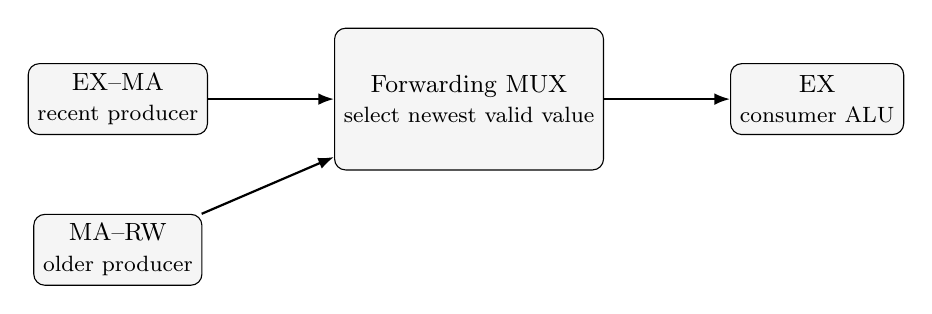
\begin{tikzpicture}[node distance=10mm]
\node[box] (exma) {EX--MA\\\footnotesize recent producer};
\node[box, below=of exma] (mabw) {MA--RW\\\footnotesize older producer};
\node[box, right=16mm of exma, minimum height=1.8cm] (mux) {Forwarding MUX\\\footnotesize select newest valid value};
\node[box, right=16mm of mux] (ex) {EX\\\footnotesize consumer ALU};
\draw[arr] (exma) -- (mux);
\draw[arr] (mabw) -- (mux);
\draw[arr] (mux) -- (ex);
\end{tikzpicture}
\captionof{figure}{Conceptual forwarding network. The MUX chooses the newest valid producer result and supplies it directly to the consumer's EX inputs.}
\end{center}

\begin{center}
\begin{tabular}{@{}L{2.6cm}L{4.6cm}L{6.4cm}@{}}
\toprule
Path & Typical use & Timing reason \\
\midrule
MA $\to$ EX & Immediate ALU-to-ALU dependency & The producer's ALU result is available after EX and is needed by the next instruction in EX. \\
RW $\to$ EX & Dependency with a larger instruction gap & The result has reached MA--RW by the time the consumer enters EX. \\
RW $\to$ OF & Operand needed during OF & Useful when a consumer needs a value during operand fetch, for example for certain branch/address computations. \\
MA $\to$ MA & Load followed by a store & Loaded data becomes available late in MA, while the store needs the data in its own MA stage. \\
\bottomrule
\end{tabular}
\captionof{table}{The forwarding paths follow from result availability and the stage at which the consumer needs the value.}
\end{center}

The important point is that forwarding is a timing mechanism, not a change to the instruction's semantics. A processor forwards the most recent value that is already available and uses normal register-file write-back for architectural state. Consequently, forwarding can remove ordinary ALU-to-ALU RAW stalls, but it cannot manufacture a value before the operation that produces it has completed. This limitation leads directly to the load-use hazard.

\subsection{The Load-Use Hazard}

The previous LOAD--STORE example showed a case in which the loaded value can reach a following instruction in time because the consumer needs it in MA. The critical case is an immediate ALU use:

\begin{lstlisting}[caption={A load-use hazard: I2 consumes I1's loaded value one cycle too early},label={lst:load-use}]
I1: ld  r6, 0[r7]
I2: add r9, r6, r8
\end{lstlisting}

Here I2 needs r6 at the beginning of EX, but I1 obtains the memory value only at the end of MA. The value is one cycle too late as a result. Even with the forwarding network above, the processor must insert one bubble\index{pipeline bubble}\glsadd{bubble} and then forward the loaded value to I2. The load-use hazard is thus the clearest example of the boundary of forwarding: if the producer has not generated the value by the time the consumer needs it, bypassing cannot remove the stall.~\cite{hennessy}

\section{Control Hazards and Branch Penalty}
\label{sec:control-hazards}

\subsection{The Problem}

Data hazards arise when an instruction needs a value that has not yet been produced by an earlier instruction. A control hazard has a similar underlying cause, but the uncertainty concerns which instruction should execute next rather than the value of an operand.

Suppose a branch instruction enters the five-stage pipeline. The processor knows the address of the sequentially following instruction immediately, so it can continue fetching instructions from that path. However, the branch's actual outcome and target are not determined until the branch reaches the Execute (EX) stage. In the five-stage pipeline considered here, this occurs in the third cycle relative to the branch's own fetch. By that time, two subsequent instructions have already entered the pipeline.

If the branch turns out to be not taken, those instructions were fetched from the correct path and can continue executing normally. If the branch is taken, however, both instructions belong to the wrong path. Allowing them to continue could produce incorrect architectural effects, such as modifying a register or memory location, before the processor has recognized that they should never have executed. They must, as a result, be cancelled and replaced by instructions from the branch target.

This situation is called a control hazard. The central problem, in short, is that the pipeline has to make a decision about the next program counter before the branch outcome is actually known. Pipelining creates the performance opportunity by fetching ahead, but that same look-ahead creates work that may have to be discarded when the control flow changes.~\cite{sarangi}

\subsection{Two Hardware Policies}

There are two straightforward ways for the hardware to deal with this uncertainty. The most conservative approach is to stall the fetch stage until the branch is resolved. In the five-stage pipeline, the processor knows the branch outcome only when it reaches EX, so instruction fetch is held for two cycles. This guarantees that no wrong-path instruction enters the pipeline, but it imposes a two-cycle cost on every branch, regardless of whether the branch is actually taken.

A more efficient approach is to predict that the branch will not be taken. Instead of waiting, the processor continues fetching the sequential instructions. If the prediction is correct, there is no correction to perform. If the branch turns out to be taken, however, the instructions fetched speculatively after the branch are discovered to be on the wrong path. They are converted into bubbles, and the fetch unit is redirected to the branch target.

For this five-stage pipeline, a taken branch under predict-not-taken\index{predict-not-taken} produces two wasted cycles as a result. The two instructions fetched before the branch resolved must be discarded. The branch penalty is consequently a direct measure of the speculative work that must be thrown away when the prediction is wrong.~\cite{sarangi}

Deeper pipelines make this effect more pronounced. If branch resolution occurs farther down the pipeline, more instructions can enter the machine before the processor discovers that the predicted path was incorrect. More speculative work must then be discarded. Thus, deeper pipelines can improve clock frequency while simultaneously increasing the cost of a branch misprediction.

\begin{center}
\begin{tabular}{lccccccc}
\toprule
& 1 & 2 & 3 & 4 & 5 & 6 & 7 \\
\midrule
Branch & IF & OF & EX & MA & RW & & \\
Sequential A & & IF & OF & \multicolumn{4}{c}{(discarded)} \\
Sequential B & & & IF & \multicolumn{4}{c}{(discarded)} \\
Target & & & & IF & OF & EX & MA \\
\bottomrule
\end{tabular}
\captionof{figure}{Predict-not-taken in the five-stage pipeline. If the branch is taken, the two sequential-path instructions already in flight are discarded when the branch resolves in EX.}
\end{center}

\subsection{The Software Alternative: Delayed Branches}

Control hazards can also be addressed partly through software rather than through additional hardware. In a delayed-branch design, the architecture defines the instructions immediately following a branch as delay slots. These instructions are guaranteed to execute regardless of whether the branch is eventually taken.

The compiler can, accordingly, attempt to fill these slots with useful instructions that would have been executed on either control-flow path. For example, an instruction that advances a pointer or updates a loop counter may be moved into a delay slot if it does not depend on the branch outcome and does not interfere with the branch's own computation.

A successful schedule converts what would otherwise have been wasted cycles into useful work. However, this approach places responsibility on the compiler. The compiler must determine whether an instruction can legally be moved into the delay slot, and there may simply be no suitable instruction available. Delayed branching represents, in this sense, a different point in the hardware-software trade-off: prediction and interlocking make decisions dynamically, whereas delayed branching exposes part of the pipeline timing to the compiler.~\cite{sarangi}

\section{A Worked Example: A Small Loop Through the Pipeline}
\label{sec:worked-example}

The interaction between data and control hazards becomes clearer when they are considered together in a small loop. Take a loop that loads successive elements of an array, accumulates them into a running sum, advances the array pointer, decrements a loop counter, compares the counter against zero, and branches back to the beginning while the loop remains active:

\begin{lstlisting}[caption={A small loop combining a load-use hazard, an ordinary RAW dependency, and a control hazard},label={lst:worked-loop}]
loop: ld   r1, 0[r2]     ; [1] load array element
      add  r6, r6, r1    ; [2] accumulate
      addi r2, r2, 4     ; [3] advance pointer
      subi r3, r3, 1     ; [4] decrement counter
      cmp  r3, r0        ; [5] compare
      bgt  loop           ; [6] branch
\end{lstlisting}

This short sequence contains several different situations developed throughout the chapter. First, instruction [2] consumes the value produced by instruction [1]. Since [1] is a load and [2] immediately uses the loaded value, this is the load-use hazard discussed earlier. Forwarding cannot completely remove this dependency, so one stall cycle remains. Second, instruction [5] depends on the value generated by instruction [4]. Unlike the load-use case, this is an ordinary ALU dependency. The result of [4] is available early enough for forwarding to supply it to [5], so this RAW dependency can be resolved without an additional stall. Finally, instruction [6] is a branch. Its outcome determines whether execution returns to \texttt{loop} or continues beyond the loop, and introduces a control hazard as a result.

\textbf{Cost with Interlocks Only.} Suppose the processor uses hardware interlocks but has no forwarding. The pipeline must wait until each producer has written its result back to the register file before allowing the dependent instruction to proceed. The dependency between [1] and [2] therefore costs three cycles. The dependency between [4] and [5] costs another three cycles. In addition, if the branch is handled conservatively by waiting for its resolution, the taken branch contributes a two-cycle penalty.

The loop contains six instructions, so six cycles would be the idealized cost of one iteration once pipeline throughput is established. The total cost becomes

\begin{equation}
6 + 3 + 3 + 2 = 14 \text{ cycles.}
\end{equation}

Thus, hazard handling increases the cost of an iteration from the ideal six cycles to fourteen cycles. The example illustrates how several individually simple hazards can combine into a substantial performance penalty.

\textbf{Cost with Forwarding and Delayed Branches.} Now consider the same loop with forwarding and delayed branches. The dependency between [4] and [5] can be resolved entirely through forwarding, so it contributes no additional cycles. The dependency between [1] and [2] remains a load-use hazard and therefore requires exactly one stall cycle.

The branch provides two delay slots. In this particular loop, instructions [3] and [4] can occupy these slots because both operations are performed on every iteration and neither depends on the outcome of the branch. The work that would otherwise have occupied the two branch-delay cycles is therefore useful computation rather than wasted time.

The resulting cost is

\begin{equation}
6 + 1 + 0 + 0 = 7 \text{ cycles per iteration.}
\end{equation}

\begin{center}
\begin{tabular}{lccccccccc}
\toprule
Instr. & 1 & 2 & 3 & 4 & 5 & 6 & 7 & 8 & 9 \\
\midrule
1: ld & IF & OF & EX & MA & RW & & & & \\
2: add & & IF & OF & STALL & EX & MA & RW & & \\
3: addi & & & IF & & OF & EX & MA & RW & \\
4: subi & & & & IF & & OF & EX & MA & RW \\
5: cmp & & & & & IF & & OF & EX & MA \\
6: bgt & & & & & & IF & & OF & EX \\
\bottomrule
\end{tabular}
\captionof{figure}{Forwarding and delayed branching reduce the loop to one unavoidable load-use stall; independent pointer and counter updates can occupy the branch-delay slots.}
\end{center}

A single iteration costs seven cycles as a result. The same loop that required fourteen cycles under interlocking alone now requires only seven cycles. The example demonstrates the combined effect of the mechanisms developed in this chapter: forwarding removes avoidable RAW stalls, while software scheduling can make otherwise wasted branch slots useful.

\begin{center}
\begin{tabular}{lccc}
\toprule
Scheme & Base cost & Hazard cost & Total \\
\midrule
Interlocks only & 6 & $3+3+2=8$ & 14 \\
Forwarding + delayed branch & 6 & $1+0+0=1$ & 7 \\
\bottomrule
\end{tabular}
\captionof{table}{Cycle cost per loop iteration under the two hazard-handling schemes.}
\end{center}

\section{Summary}
\label{sec:ch2-summary}

A five-stage pipeline improves instruction throughput by allowing different instructions to occupy different stages simultaneously. However, the overlap that produces this performance benefit also creates situations in which instructions cannot simply proceed independently. The processor must preserve correctness while attempting to maintain as much overlap as possible.

Data hazards arise when an instruction requires a value that an earlier instruction has not yet made available. In the in-order pipeline considered here, the relevant dependency is RAW because instructions cannot overtake one another. Hardware interlocks provide a general solution by detecting dependencies and stalling the pipeline, but they can introduce unnecessary delays. Forwarding\index{forwarding}\glsadd{forwarding} improves this situation by allowing already-computed results to be transferred directly between pipeline stages. It eliminates the cost of ordinary RAW dependencies in this five-stage design, but it cannot remove the load-use hazard\index{hazard!load-use}\glsadd{loaduse} because a load's result does not exist early enough for an immediately following ALU instruction.~\cite{sarangi}

Control hazards\index{hazard!control} arise from a different kind of uncertainty: the processor does not know the correct next instruction until a branch is resolved. A conservative stall guarantees correctness but wastes cycles on every branch. Predict-not-taken allows the pipeline to continue speculatively and pays a penalty only when the branch is actually taken. Delayed branching\index{delayed branch}\glsadd{delayedbranch} provides a software alternative in which the compiler attempts to fill the otherwise wasted slots with useful instructions.~\cite{sarangi}

The worked loop demonstrates the combined effect. A pipeline without forwarding or effective branch scheduling can lose a large fraction of its potential throughput to hazards. Introducing forwarding and making useful use of branch-delay slots reduces this overhead substantially. The broader lesson is that pipelining is not merely a matter of dividing instruction execution into stages. Its performance depends on how effectively the processor and compiler manage the dependencies and control-flow uncertainty created by having several instructions in flight at once.

This also sets up the next chapter naturally. The mechanisms considered here use relatively simple, fixed policies: stall for a known dependency, forward an available result, or use a simple branch policy such as predict-not-taken. The next step is to ask what happens when the processor attempts to make these decisions more intelligently at run time. This leads to branch prediction, wider issue, out-of-order execution, register renaming, and speculative execution, which allow the processor to extract more instruction-level parallelism while managing increasingly complex forms of uncertainty. The software side of the same problem returns later through compiler scheduling, where the manual instruction rearrangement illustrated by this loop becomes a systematic compile-time technique.~\cite{sarangi}



% =======================================================================
%  APPENDICES: plagiarism report, reading indices, progress report
%  (required for this submission), and the forward plan for
%  submissions 2--4.
% =======================================================================
\appendix

\chapter{Plagiarism Report}
\label{app:plagiarism}

\section{Summary of the Generated Report}
\label{sec:plagiarism-summary}

A preliminary similarity and writing-quality check was run on the
compiled draft using Grammarly. Across the submitted text (15,389 words, 965
sentences), the tool reported an overall writing score of 85/100,
placing the draft above 85\% of texts it evaluates, with 376 writing
issues flagged (263 critical, 113 advanced) for the team to review
before the deliverable is finalised. On originality, the check found
2\% textual overlap with 54 sources drawn from the web and academic
archives, consistent with the paper's citation-heavy style, in which
the text closely paraphrases and correctly attributes established
results (for example Tomasulo's algorithm and the RISC design
philosophy) rather than reproducing them verbatim. This 2\% figure is
expected to overlap substantially with the sources already cited in
\cref{ch:intro,ch:pipeline-basics} and should be treated as a
preliminary indicator only; the authoritative similarity figure for
this submission remains the institute-approved report described above.

\begin{center}
% Link to the original plagiarism report image (disabled in the
% compiled PDF; kept here in the source for reference / re-enabling):
% \href{run:plagiarism_report.png}{\textbf{View the original plagiarism report image}}\\[6pt]
% \href{run:plagiarism_report.png}{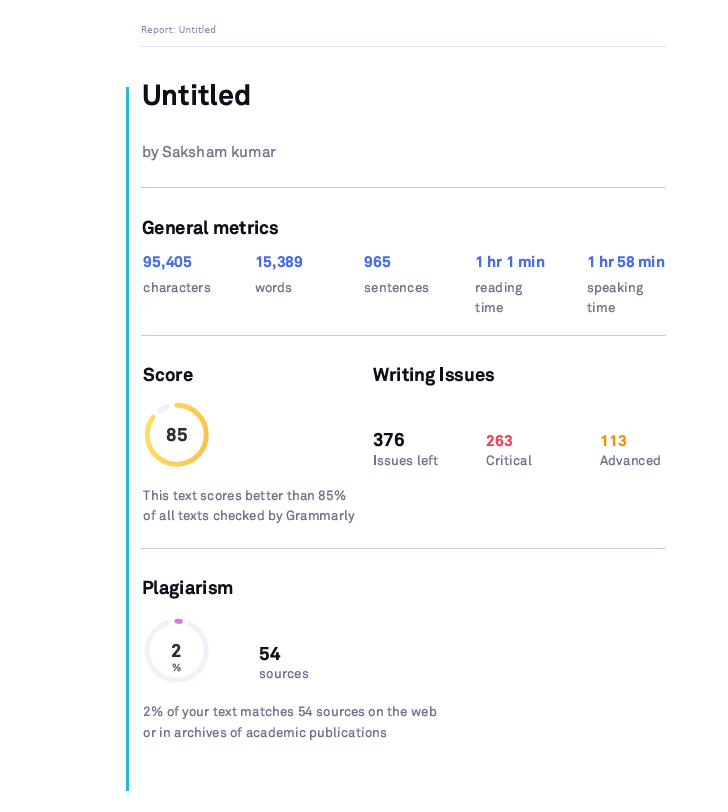
\includegraphics[width=0.75\textwidth]{plagiarism_report.png}}
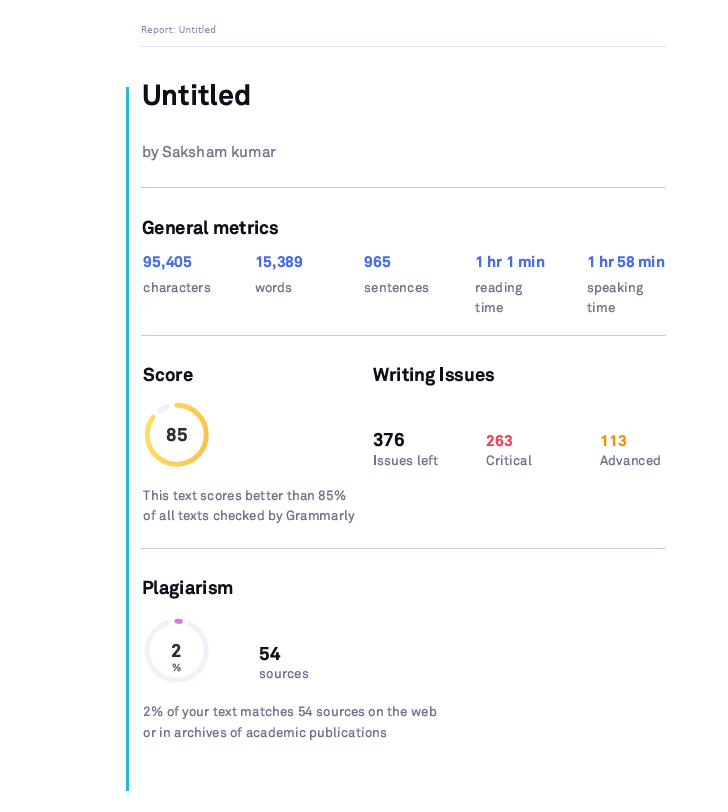
\includegraphics[width=0.75\textwidth]{plagiarism_report.png}
\end{center}

\chapter{Reading Indices}
\label{app:readability}

This appendix reports standard automated readability indices for the
written prose of this draft (\cref{ch:intro,ch:pipeline-basics}),
computed directly from the submitted text using the open-source
\texttt{textstat} library, which implements the same formulas
documented at
\url{https://www.analyzemywriting.com/readability_indices.html}. Tables,
equations, code listings, and citation markup were stripped before
computing these figures, so that only prose contributes to the word,
sentence, and syllable counts each index is built from.

\begin{table}[htbp]
\centering
\caption{Automated readability indices computed on the full written
portion of this draft (\Cref{ch:intro,ch:pipeline-basics} combined,
7{,}035 words, 335 sentences).}
\label{tab:readability}
\begin{tabular}{@{}L{0.55\textwidth}L{0.15\textwidth}L{0.2\textwidth}@{}}
\toprule
\textbf{Index} & \textbf{Score} & \textbf{Interpretation} \\
\midrule
Flesch Reading Ease & 34.8 & Difficult (college level) \\
Flesch--Kincaid Grade Level & 13.6 & 13th--14th grade \\
Gunning Fog Index & 17.0 & Graduate reading level \\
SMOG Index & 15.7 & 15th--16th grade \\
Coleman--Liau Index & 14.3 & College level \\
Automated Readability Index & 15.3 & College level \\
Dale--Chall Readability Score & 11.3 & College graduate \\
Linsear Write Formula & 10.9 & 11th grade \\
\bottomrule
\end{tabular}
\end{table}

\begin{table}[htbp]
\centering
\caption{Supporting statistics for the indices above.}
\label{tab:readability-stats}
\begin{tabular}{@{}L{0.55\textwidth}L{0.35\textwidth}@{}}
\toprule
\textbf{Statistic} & \textbf{Value} \\
\midrule
Word count & 7{,}035 \\
Sentence count & 335 \\
Syllable count & 12{,}535 \\
Average sentence length & 21.0 words \\
Average syllables per word & 1.78 \\
Estimated reading time & $\sim$9.6 minutes \\
\bottomrule
\end{tabular}
\end{table}

\Cref{tab:readability-breakdown} splits the two written chapters apart,
since they differ somewhat in style: \cref{ch:intro} is argumentative
and equation-adjacent prose, while \cref{ch:pipeline-basics} is more
procedural, walking through mechanisms step by step, which is reflected
in its slightly lower grade-level scores.

\begin{table}[htbp]
\centering
\caption{Readability by chapter.}
\label{tab:readability-breakdown}
\begin{tabular}{@{}L{0.32\textwidth}L{0.14\textwidth}L{0.24\textwidth}L{0.14\textwidth}@{}}
\toprule
\textbf{Chapter} & \textbf{Words} & \textbf{Flesch Reading Ease} & \textbf{F--K Grade} \\
\midrule
\Cref{ch:intro} & 2{,}234 & 32.7 & 15.5 \\
\Cref{ch:pipeline-basics} & 4{,}801 & 34.8 & 13.1 \\
\bottomrule
\end{tabular}
\end{table}

\noindent\textbf{Interpretation.} All indices place this draft at
upper-undergraduate to graduate reading level, which is expected and
appropriate for a technical term paper aimed at students who have
already taken the prerequisite architecture lectures: the vocabulary
includes domain terms (hazard, forwarding, AMAT) that these formulas
count as long, complex words regardless of how familiar they are to the
paper's actual intended reader. The Flesch Reading Ease score of 34.8
falls in the ``difficult'' band on the standard 0--100 scale, consistent
with a document that derives results algebraically and defines terms
precisely rather than writing for a general audience. These figures will
be recomputed for the final submission once all technical chapters are
complete, since chapters with denser mathematical notation are expected
to raise the grade-level estimates further.

\chapter{Extended Historical Discussion}
\label{app:history}

\Cref{ch:intro} keeps its central argument to the two stall equations,
\cref{eq:mem-stall,eq:branch-stall}, and to the structural claim that
pipelining, memory hierarchy, and compiler scheduling are three levers
on those equations rather than three unrelated syllabus topics. The
historical material that motivates and supports that argument, but is
not itself required to follow it, is collected here instead of
interrupting the chapter's main line of reasoning.

\section{Why This Trio Became Unavoidable}
\label{app:history-trio}

This trio of problems is not a recent invention, but the particular
urgency with which architects have had to confront it together is. For
roughly three decades after the invention of the integrated circuit,
\gls{dennard}\index{Dennard scaling} meant that each new process generation delivered
transistors that were not only smaller but also faster and lower in
power, so that clock frequency could rise from one generation to the
next largely for free. Architects could treat memory latency and branch
misprediction cost as problems a faster clock would eventually shrink in
absolute terms, even while the underlying cycle counts stayed roughly
the same. That free lunch ended in the middle of the 2000s. Dennard
scaling broke down once leakage current and power density stopped
shrinking in step with transistor size, and single-thread clock
frequency plateaued across the industry at a few gigahertz. The
industry's response was the shift to multicore designs: rather than
making one core faster, manufacturers began placing several cores on a
die and asking software to keep all of them busy \cite{esmaeilzadeh2011}.

That shift changed the stakes of everything this paper studies. A single
core's memory stalls no longer shrink automatically with each process
generation the way they once implicitly did while clock speed alone was
rising. Multiple cores now compete for the same shared off-chip memory
bandwidth, turning the single-core memory wall identified by Wulf and
McKee into a contended, shared resource rather than a private one
\cite{wulfmckee1995}. And because per-core performance can no longer be
bought simply by raising the clock, the incremental gains available from
a better pipeline, a better memory hierarchy, and better compiler
scheduling are, in a fairly literal sense, most of what remains on the
table. The three parts of this paper are not an arbitrary partition of a
broad syllabus. They are close to the complete list of levers an
architect still has, now that the easiest lever, clock frequency, has
largely been used up.

\section{The Historical Origins of Each Pillar's Difficulty}
\label{app:history-pillars}

\subsection{Pipeline Correctness: Tomasulo and the RISC Philosophy}

This difficulty predates the five-stage pipeline studied in this paper
by several decades. As soon as machines moved from single-cycle
execution toward pipelined and eventually multiple-issue implementation,
correctness in the presence of hazards became a first-class design
constraint rather than an afterthought. Tomasulo's algorithm\index{Tomasulo's algorithm}, developed
for the IBM System/360 Model 91 in the 1960s, was an early and
influential answer to precisely this problem in a machine with several
independent execution units: it showed that hardware could look several
instructions ahead, resolve data dependences dynamically through a
shared common data bus, and still guarantee the same result a strictly
sequential machine would have produced \cite{tomasulo1967}. The
instruction set decisions that make a simple pipeline tractable in the
first place, particularly the choice to confine memory access to
dedicated load and store instructions, trace back to the reduced
instruction set philosophy that Patterson and Ditzel argued for
explicitly in 1980, on the grounds that simple, uniform instructions are
what make a clean pipeline implementation possible at all
\cite{pattersonditzel1980}. \Cref{ch:pipeline-basics} develops the
pipeline that decision makes possible, and \cref{ch:branch-ooo} develops
the dynamic techniques, descended in spirit from Tomasulo's original
scheme, that let a modern core go well beyond it.

\subsection{The Memory Hierarchy: Denning, Mattson, and Wulf--McKee}

The empirical shape of this problem was established well before the
transistor budgets of modern chips made it as severe as it now is.
Denning's \gls{workingset}\index{working set} model, published in 1968, gave the first rigorous
account of why a small, fast memory can nonetheless serve most of a
program's references most of the time: programs concentrate their
accesses on a slowly changing subset of their address space, and a cache
sized to hold that subset captures nearly all the benefit a much larger
cache would provide \cite{denning1968}. Mattson, Gecsei, Slutz, and
Traiger formalised this two years later with reuse-distance analysis,
showing that a single pass over a program's memory trace could
determine the hit rate of a fully associative cache at every possible
capacity simultaneously \cite{mattson1970}. Wulf and McKee's 1995 note,
already introduced above, gave the resulting and widening gap between
processor and memory speed its now-standard name, the \gls{memorywall}\index{memory wall}
\cite{wulfmckee1995}. The chapters of \cref{part:memory} are, in a
real sense, an extended answer to the question those papers first posed
together: given that locality is real and that memory is slow, what
structure should a memory system actually have, and how far can that
structure be pushed once several cores must share it?

\subsection{Compile-Time Scheduling: Fisher and the ELI-512}

This gap is not merely theoretical. Fisher's work on the ELI-512 in the
early 1980s demonstrated that a sufficiently aggressive compiler could
extract far more instruction-level parallelism from ordinary code than
had previously been assumed possible, provided the hardware was willing
to trust the compiler's schedule completely and dispense with the
dynamic hazard-checking machinery that \cref{part:pipeline} develops
\cite{fisher1983}. That single design choice, whether to trust a static
schedule outright or to verify everything again at run time, turns out
to be one of the more consequential decisions in the history of
processor design, and \cref{ch:ilp-philosophy} returns to it directly by
placing VLIW and superscalar execution side by side.

% =======================================================================
%  The following two appendices (D, E) were prepared for Submission 1
%  as a progress report and forward plan and are retained in that role.
% =======================================================================

\chapter{Work Done as of 24 August 2026}
\label{app:progress}

This appendix is the progress report required for Submission~1. It
states the chosen topic, maps it onto the prescribed textbook, records
which faculty advisor the team will consult, breaks the remaining work
into work packages and dated tasks with a percentage completion for
each, presents that schedule as a Gantt chart
(\cref{fig:gantt}), and documents how the bibliography is being managed.

\section{The Chosen Topic}
\label{sec:topic}

The topic of this term paper is \emph{modern processor
microarchitecture, treated as a single performance problem with three
coupled levers}: the instruction pipeline, the memory hierarchy, and the
compiler that targets both.

The framing, argued quantitatively in \cref{sec:central-problem}, is
that these three subjects are usually taught as separate chapters but
are in fact three ways of acting on the same two stall equations,
\cref{eq:mem-stall,eq:branch-stall}. The paper's contribution is
therefore not a survey of three topics but a unified derivation: hazards
are shown to \emph{force} forwarding and stalling; the circuit-level
behaviour of SRAM and DRAM cells is shown to \emph{force} a layered
hierarchy; and the compiler's static visibility into a program is shown
to \emph{force} particular scheduling choices. The paper closes by
tracing one benchmark through all three mechanisms on two real
architectures and testing whether the models derived earlier actually
predict what hardware performance counters report.

The work is divided across three authors, one per technical pillar, with
the introduction, the synthesis chapter and the final integration
written jointly. \Cref{tab:author-split} records the division.

\begin{table}[htbp]
\centering
\caption{Division of work across the three authors.}
\label{tab:author-split}
\begin{tabular}{@{}L{0.18\textwidth}L{0.34\textwidth}L{0.38\textwidth}@{}}
\toprule
\textbf{Author} & \textbf{Primary responsibility} & \textbf{Chapters} \\
\midrule
Author~1 & Pipelining and instruction execution &
  \Cref{ch:pipeline-basics,ch:branch-ooo} \\
Author~2 & The memory hierarchy &
  \Cref{ch:memcells,ch:caches,ch:coherence} \\
Author~3 & Compiler--architecture co-design &
  \Cref{ch:compiler-sched,ch:regalloc,ch:ilp-philosophy} \\
All three & Framing, synthesis, measurement, integration &
  \Cref{ch:intro,ch:synthesis,ch:conclusion} \\
\bottomrule
\end{tabular}
\end{table}

\section{Mapping to the Prescribed Textbook}
\label{sec:app-textbook}

The topic maps principally onto three chapters of Sarangi,
\emph{Basic Computer Architecture} \cite{sarangi}:

\begin{itemize}[leftmargin=*]
  \item \textbf{Chapter~10, \emph{Principles of Pipelining}} --- the
    anchor chapter for \cref{ch:pipeline-basics} (\S10.1--\S10.6: the
    pipelined datapath, the five IF/OF/EX/MA/RW stages, pipeline
    registers and the instruction packet, and the structural, data and
    control hazards with their interlock and forwarding solutions) and
    for \cref{ch:branch-ooo} (\S10.9: branch prediction, multiple-issue
    in-order pipelines, EPIC/VLIW, and out-of-order pipelines). \S10.7,
    on the inter-relationship between performance, the compiler,
    architecture and technology, is the textbook's only direct hook for
    \cref{ch:compiler-sched}.
  \item \textbf{Chapter~11, \emph{The Memory System}} --- the anchor
    chapter for \cref{ch:memcells,ch:caches,ch:coherence} (\S11.1
    overview, \S11.2 caches, \S11.3 the mathematical model of the memory
    system, \S11.4 virtual memory), supported by Chapter~9, \S9.4
    \emph{Memories} for the SRAM/DRAM/CAM cell-level material that
    \cref{ch:memcells} needs.
  \item \textbf{Chapter~12, \emph{Multiprocessor Systems}} --- coherence
    and memory consistency, for the multicore half of
    \cref{ch:coherence}; and \textbf{Appendix~A}, the case studies of
    real processors, for \cref{ch:synthesis}.
\end{itemize}

The chapter-by-chapter correspondence, including section and page
ranges, is given in full in \cref{tab:textbook-map}. The only part of the paper that the prescribed
text does not substantially cover is \cref{part:compiler}, and
\cref{ch:regalloc} in particular; that material is developed from
\cite{hennessy} and Shen and Lipasti
\cite{shen} instead, which is why the reading load in WP2 below is
weighted toward Author~3.

\paragraph{Faculty advisor.} As advised, the team will consult
\textbf{Prof.\ Subrat Kar} on this term paper. The shared Zotero group
library described in \cref{sec:zotero} has been created with
Prof.\ Subrat Kar added as a member, so that the reference list and the
stored PDFs are visible without a separate submission step.

\section{Work Packages and Task Status}
\label{sec:workpackages}

The remaining work is organised into four work packages. WP1 is
prescribed-text reading, WP2 is external literature and reference
management, WP3 is writing, and WP4 is the experimental and synthesis
work that \cref{ch:synthesis} depends on. Percentages below are measured
against the deliverable named in the task, not against elapsed time.

\subsection*{WP1 --- Reading the prescribed text}
\begin{itemize}[leftmargin=*]
  \item \textbf{Task~1.1.} Read Ch.~10, \emph{Principles of Pipelining},
    \S10.1--\S10.6 (pp.~413--457) from the text \cite{sarangi}, by
    18~Aug 2026: \textbf{100\% done}. This reading is what
    \cref{ch:pipeline-basics} of this submission is built on.
  \item \textbf{Task~1.2.} Read Ch.~10, \S10.7 and \S10.9,
    \emph{Advanced Techniques} (pp.~476, 487--497), by 31~Aug 2026:
    \textbf{45\% done}. Feeds \cref{ch:branch-ooo,ch:ilp-philosophy}.
  \item \textbf{Task~1.3.} Read Ch.~9, \S9.4 \emph{Memories}
    (pp.~288--297) and Ch.~11, \S11.1--\S11.3 (pp.~508--541), by
    14~Sep 2026: \textbf{30\% done}. Feeds
    \cref{ch:memcells,ch:caches}.
  \item \textbf{Task~1.4.} Read Ch.~11, \S11.4 \emph{Virtual Memory},
    Ch.~12, \S12.4 \emph{Coherence and Consistency}, and Appendix~A
    (case studies of real processors), by 5~Oct 2026:
    \textbf{0\% done}. Feeds \cref{ch:coherence,ch:synthesis}.
\end{itemize}

\subsection*{WP2 --- External literature and reference management}
\begin{itemize}[leftmargin=*]
  \item \textbf{Task~2.1.} Create the shared Zotero group library, agree
    a citation-key convention, and share the library with
    Prof.\ Subrat Kar: \textbf{100\% done}. See \cref{sec:zotero}.
  \item \textbf{Task~2.2.} Read papers related to the topic and store
    the references \emph{and} the PDFs in Zotero:
    \textbf{18 references read and filed so far}, cited individually
    throughout \cref{ch:intro,ch:pipeline-basics} and listed in full in
    the consolidated bibliography at the end of this document. Target for
    Submission~2: \textbf{30\% done}.
  \item \textbf{Task~2.3.} Add at least 15 further references covering
    compiler scheduling, register allocation and VLIW/EPIC, which the
    prescribed text does not cover, by 19~Oct 2026:
    \textbf{5\% done}.
\end{itemize}



\subsection*{WP3 --- Writing, chapter development and research integration}
\begin{itemize}[leftmargin=*]
  \item \textbf{Task~3.1.} Write \cref{ch:intro} (Introduction), fixing
    the paper's thesis, notation, non-aims and textbook mapping:
    \textbf{100\% done} --- delivered in this submission.

  \item \textbf{Task~3.2.} Write \cref{ch:pipeline-basics} (Instruction
    Set Design and Pipelining), including the worked examples and
    pipeline analysis: \textbf{100\% done} --- delivered in this
    submission.

  \item \textbf{Task~3.3.} Research and begin drafting
    \cref{ch:branch-ooo} (Branch Prediction and Out-of-Order
    Execution). This includes reading the relevant prescribed-text
    sections, reviewing the main concepts needed for dynamic branch
    prediction, register renaming and out-of-order execution, and
    developing the chapter structure before completing the prose. By
    21~Sep 2026: \textbf{10\% done}.

  \item \textbf{Task~3.4.} Research and develop
    \cref{ch:memcells,ch:caches,ch:coherence} (the memory hierarchy).
    This includes reading the relevant chapters and sections of the
    prescribed text, consolidating the terminology and concepts,
    planning the relationship between memory cells, caches, virtual
    memory, coherence and consistency, and then drafting the chapters.
    By 19~Oct 2026: \textbf{5\% done}.

  \item \textbf{Task~3.5.} Research and develop
    \cref{ch:compiler-sched,ch:regalloc,ch:ilp-philosophy} (compiler
    co-design). Work includes reading the relevant prescribed-text
    sections, identifying the material that must be supplemented by
    external reading, organising the chapter structure, and developing
    the explanations of scheduling, register allocation and VLIW/EPIC.
    By 26~Oct 2026: \textbf{5\% done}.

  \item \textbf{Task~3.6.} Maintain a running chapter outline and
    research notes for the remaining chapters, recording definitions,
    examples, figures, open questions and connections between the
    three technical pillars. Update the outline as reading and
    research progress: \textbf{ongoing}.

  \item \textbf{Task~3.7.} Integrate completed research into the
    written chapters, checking that claims, terminology, examples and
    internal cross-references remain consistent as later chapters are
    added: \textbf{ongoing}.
\end{itemize}

\subsection*{WP4 --- Experiments, analysis, synthesis and integration}
\begin{itemize}[leftmargin=*]
  \item \textbf{Task~4.1.} Plan and implement the latency-staircase
    microbenchmark: a pointer-chasing walk over geometrically
    increasing working-set sizes to identify cache-level boundaries on
    a real machine. Select the test machine, define the measurement
    procedure, run repeated trials, and collect the latency data using
    Intel VTune where appropriate. By 5~Oct 2026: \textbf{0\% done}.

  \item \textbf{Task~4.2.} Develop and validate the trace-driven cache
    simulator. Generate representative memory traces using DynamoRIO
    or Pin, implement the required cache configurations, and use the
    resulting simulations to analyse the compulsory, capacity and
    conflict components of cache misses. By 19~Oct 2026:
    \textbf{0\% done}.

  \item \textbf{Task~4.3.} Analyse the experimental results and compare
    them with the predictions developed in \cref{ch:memcells,ch:caches}.
    Record cache capacities, observed latency transitions, miss-rate
    behaviour and any discrepancies between the expected and measured
    results: \textbf{0\% done}.

  \item \textbf{Task~4.4.} Write \cref{ch:synthesis}, using the
    experimental results to connect the three main mechanisms studied
    in the paper. State the predicted behaviour first, present the
    measured results, and then explain significant agreements or
    divergences: by 2~Nov 2026: \textbf{0\% done}.

  \item \textbf{Task~4.5.} Perform the final integration pass across
    the paper. Check notation, terminology, chapter transitions,
    figures, tables, bibliography entries and all internal
    cross-references, and ensure that the experimental discussion is
    consistent with the theoretical chapters. By 9~Nov 2026:
    \textbf{0\% done}.

  \item \textbf{Task~4.6.} Conduct a final consistency and quality
    review of the complete paper, including checking that the planned
    arguments are supported by the research completed, that
    experimental claims are reproducible from the described procedure,
    and that the final chapter structure remains coherent:
    \textbf{0\% done}.
\end{itemize}




\section{Progress Gantt Chart}
\label{sec:gantt}

\Cref{fig:gantt} presents the current work schedule as a Gantt chart.
It is drawn programmatically in TikZ, in keeping with the requirement
that every figure in this paper be generated in \LaTeX{} rather than
imported. Each bar spans the planned window for a task; the solid
portion indicates the work completed as of 24~August~2026, while the
pale remainder represents work still outstanding. The vertical dashed
lines indicate the planned submission milestones.

\begin{figure}[!htbp]
\centering
\resizebox{\textwidth}{!}{%
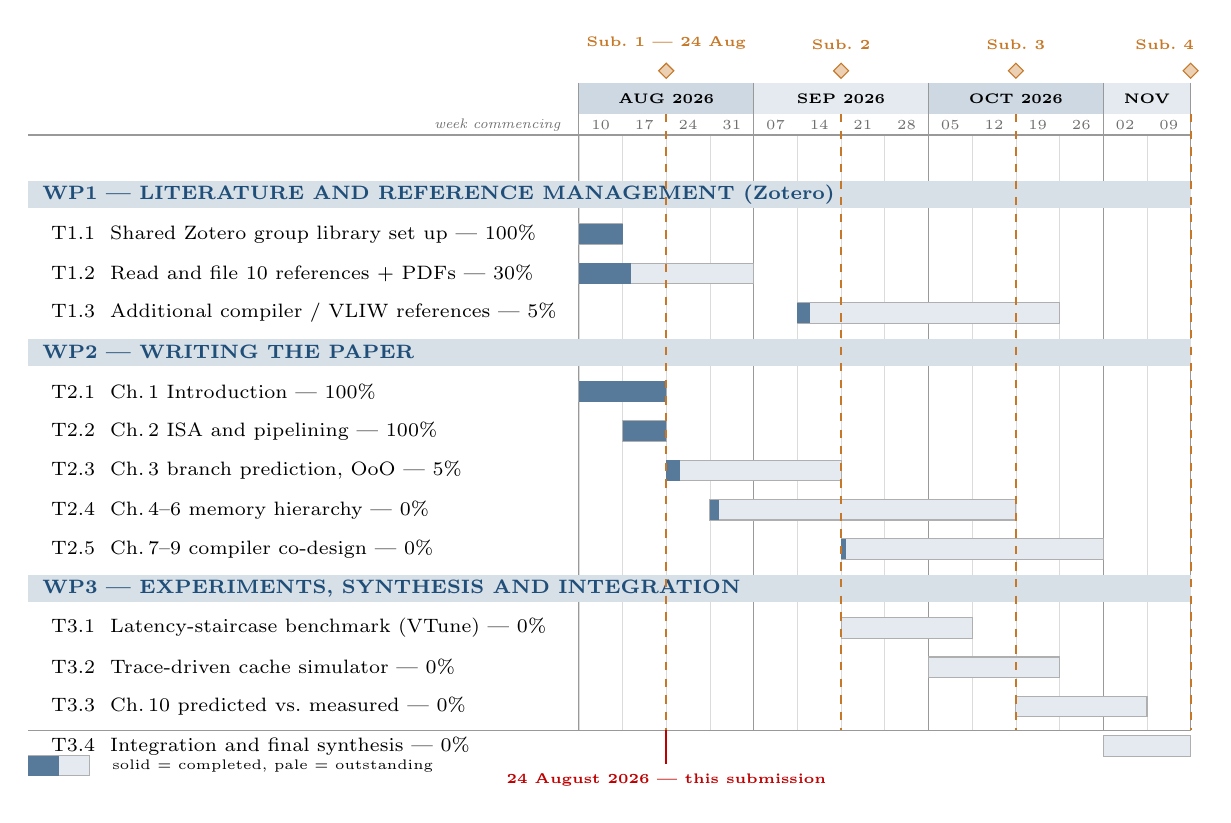
\begin{tikzpicture}[x=0.555cm,y=0.50cm]

  % ---------- month bands -------------------------------------------
  \fill[archblue!22] (0,1.05) rectangle (4,1.85);
  \fill[archblue!12] (4,1.05) rectangle (8,1.85);
  \fill[archblue!22] (8,1.05) rectangle (12,1.85);
  \fill[archblue!12] (12,1.05) rectangle (14,1.85);
  \node[font=\tiny\bfseries] at (2,1.45)  {AUG 2026};
  \node[font=\tiny\bfseries] at (6,1.45)  {SEP 2026};
  \node[font=\tiny\bfseries] at (10,1.45) {OCT 2026};
  \node[font=\tiny\bfseries] at (13,1.45) {NOV};

  % ---------- week-commencing labels --------------------------------
  \foreach \i/\d in {1/10,2/17,3/24,4/31,5/07,6/14,7/21,8/28,
                     9/05,10/12,11/19,12/26,13/02,14/09}
    \node[font=\tiny, archgray] at (\i-0.5,0.78) {\d};
  \node[anchor=east, font=\tiny\itshape, archgray] at (-0.2,0.78)
    {week commencing};

  % ---------- grid ---------------------------------------------------
  \foreach \i in {0,...,14}
    \draw[archgray!25, very thin] (\i,0.52) -- (\i,-14.60);
  \foreach \i in {0,4,8,12,14}
    \draw[archgray!70] (\i,1.85) -- (\i,-14.60);
  \draw[archgray!70] (\ganttleft,0.52) -- (14,0.52);
  \draw[archgray!70] (\ganttleft,-14.60) -- (14,-14.60);

  % ---------- literature and reference management -------------------
  \wpheader{1}{WP1 --- LITERATURE AND REFERENCE MANAGEMENT (Zotero)}
  \gtask{2}{0}{1}{1.00}{T1.1\ \ Shared Zotero group library set up --- 100\%}
  \gtask{3}{0}{4}{0.30}{T1.2\ \ Read and file 10 references + PDFs --- 30\%}
  \gtask{4}{5}{11}{0.05}{T1.3\ \ Additional compiler / VLIW references --- 5\%}

  % ---------- writing the paper -------------------------------------
  \wpheader{5}{WP2 --- WRITING THE PAPER}
  \gtask{6}{0}{2}{1.00}{T2.1\ \ Ch.\,1 Introduction --- 100\%}
  \gtask{7}{1}{2}{1.00}{T2.2\ \ Ch.\,2 ISA and pipelining --- 100\%}
  \gtask{8}{2}{6}{0.08}{T2.3\ \ Ch.\,3 branch prediction, OoO --- 5\%}
  \gtask{9}{3}{10}{0.03}{T2.4\ \ Ch.\,4--6 memory hierarchy --- 0\%}
  \gtask{10}{6}{12}{0.02}{T2.5\ \ Ch.\,7--9 compiler co-design --- 0\%}

  % ---------- experiments, synthesis and integration ----------------
  \wpheader{11}{WP3 --- EXPERIMENTS, SYNTHESIS AND INTEGRATION}
  \gtask{12}{6}{9}{0.00}{T3.1\ \ Latency-staircase benchmark (VTune) --- 0\%}
  \gtask{13}{8}{11}{0.00}{T3.2\ \ Trace-driven cache simulator --- 0\%}
  \gtask{14}{10}{13}{0.00}{T3.3\ \ Ch.\,10 predicted vs.\ measured --- 0\%}
  \gtask{15}{12}{14}{0.00}{T3.4\ \ Integration and final synthesis --- 0\%}

  % ---------- submission milestones ----------------------------------
  \foreach \x in {2,6,10,14}{
    \draw[archorange, dashed, thick] (\x,1.05) -- (\x,-14.60);
    \node[diamond, draw=archorange, fill=archorange!35, inner sep=1.4pt]
      at (\x,2.15) {};}
  \node[font=\tiny\bfseries, archorange, anchor=south] at (2,2.45)
    {Sub.\ 1 --- 24 Aug};
  \node[font=\tiny\bfseries, archorange, anchor=south] at (6,2.45)
    {Sub.\ 2};
  \node[font=\tiny\bfseries, archorange, anchor=south] at (10,2.45)
    {Sub.\ 3};
  \node[font=\tiny\bfseries, archorange, anchor=south east] at (14.3,2.45)
    {Sub.\ 4};

  % ---------- "today" marker -----------------------------------------
  \draw[red!75!black, thick] (2,-14.60) -- (2,-15.45);
  \node[font=\tiny\bfseries, red!75!black, anchor=north] at (2,-15.45)
    {24 August 2026 --- this submission};

  % ---------- legend -------------------------------------------------
  \draw[archgray!55, fill=archblue!12] (\ganttleft,-15.25) rectangle
    ({\ganttleft+1.4},-15.75);
  \fill[archblue!75] (\ganttleft,-15.25) rectangle
    ({\ganttleft+0.7},-15.75);
  \node[anchor=west, font=\tiny] at ({\ganttleft+1.7},-15.50)
    {solid = completed, pale = outstanding};

\end{tikzpicture}}
\caption{Gantt chart of the term-paper schedule, showing progress as of
24~August~2026. Horizontal units are calendar weeks, with the number
under each column indicating the Monday of that week. The dates of
Submissions~2--4 are provisional and will be aligned with the course
calendar as it is announced.}
\label{fig:gantt}
\end{figure}



\section{Bibliography and Citation Management}
\label{sec:zotero}

All references and citations for this term paper are managed in
\href{https://www.zotero.org/}{Zotero}, in a shared group library to
which all three authors and Prof.\ Subrat Kar have access. Every item in
the library carries its PDF attachment where one is available, together
with the DOI or ISBN, so that the group library is the single source of
truth for the paper's bibliography rather than any individual author's
local notes. The library is exported to a BibTeX \texttt{.bib} file,
which is what generates the consolidated bibliography at the end of this
document.

Two working rules keep the exported file usable. First, citation keys
follow a fixed \texttt{authoryear} convention (for example
\texttt{wulfmckee1995}), set in Zotero rather than edited by hand after
export, so that keys never drift between authors. Second, no reference
is cited in the paper until it has been read and filed in the group
library with its PDF, which is why the reference count reported in
Task~2.2 is a count of items \emph{read}, not merely collected.




\chapter{Plan for Submissions 2--4}
\label{app:plan}

% ---------------------------------------------------------------------
% Reserve the numbers of the chapters and parts that Chapter 1 refers
% to but which are not written yet, so that every \cref in this draft
% typesets the number the final paper will actually use.  These macros
% print nothing.
% ---------------------------------------------------------------------
\planptlabel{part:pipeline}{2}%
\planptlabel{part:memory}{3}%
\planptlabel{part:compiler}{4}%
\planptlabel{part:synthesis}{5}%
\planchlabel{ch:branch-ooo}{3}%
\planchlabel{ch:memcells}{4}%
\planchlabel{ch:caches}{5}%
\planchlabel{ch:coherence}{6}%
\planchlabel{ch:compiler-sched}{7}%
\planchlabel{ch:regalloc}{8}%
\planchlabel{ch:ilp-philosophy}{9}%
\planchlabel{ch:synthesis}{10}%
\planchlabel{ch:conclusion}{11}%

This appendix records what the remaining three submissions will contain.
It exists so that the full intended scope of the paper is visible now,
at Submission~1, rather than emerging one draft at a time, and so that
the chapter numbers used in the cross-references throughout
\cref{ch:intro} already refer to a fixed, agreed structure. Drafts are
cumulative: each submission contains everything in the previous one plus
the new chapters listed here.

\section{Chapter Plan and Page Budget}
\label{sec:plan-chapters}

\Cref{tab:page-budget} lists every chapter of the final paper, the
submission in which it is due, and its target length. The budget sums to
approximately 150 pages, the target stated in \cref{sec:organisation}.

\begin{table}[htbp]
\centering
\caption{Planned chapters, delivery submission, and target page budget.
Chapters~1 and~2 are complete as of this submission.}
\label{tab:page-budget}
\begin{tabular}{@{}L{0.42\textwidth}ccL{0.26\textwidth}@{}}
\toprule
\textbf{Chapter} & \textbf{Due in} & \textbf{Pages} & \textbf{Status} \\
\midrule
Ch.~1 Introduction & Sub.~1 & 14 & Complete \\
Ch.~2 Instruction Set Design and Pipelining & Sub.~1 & 16 & Complete \\
\midrule
Ch.~3 Branch Prediction and Out-of-Order Execution & Sub.~2 & 20 & 20\% \\
Ch.~4 Memory Cells and the Case for a Hierarchy & Sub.~2 & 14 & 15\% \\
Ch.~5 Cache Organisation and Optimisation & Sub.~3 & 22 & 10\% \\
Ch.~6 Multicore Memory: Coherence, Consistency and Prefetching & Sub.~3 & 20 & 5\% \\
\midrule
Ch.~7 Static Scheduling and Loop Transformations & Sub.~3 & 14 & 5\% \\
Ch.~8 Register Allocation and Backend Code Generation & Sub.~4 & 12 & Not started \\
Ch.~9 VLIW versus Superscalar & Sub.~4 & 10 & Not started \\
\midrule
Ch.~10 Synthesis: One Benchmark, Three Mechanisms & Sub.~4 & 12 & Not started \\
Ch.~11 Open Problems and Concluding Remarks & Sub.~4 & 6 & Not started \\
\midrule
\textbf{Total} & & \textbf{160} & \\
\bottomrule
\end{tabular}
\end{table}

\section{What Each Submission Will Add}
\label{sec:plan-submissions}

\paragraph{Submission~2.} Adds \cref{ch:branch-ooo} and
\cref{ch:memcells}. \Cref{ch:branch-ooo} relaxes the two constraints
that made \cref{ch:pipeline-basics} tractable: the fixed
predict-not-taken policy is replaced by dynamic predictors, including
bimodal, two-level, tournament, and more advanced history-based
designs, and the in-order constraint that made WAW and WAR hazards
impossible is dropped, which forces register renaming, reservation
stations, and a reorder buffer. \cref{ch:memcells} opens
\cref{part:memory} by deriving, from the six-transistor SRAM cell and
the one-transistor DRAM cell, why latency, capacity and cost per bit
cannot be optimised simultaneously, with static-noise-margin analysis
providing the quantitative core and DRAM reliability providing a
concrete example of the trade-off that arises when density is pushed
too far.

\paragraph{Submission~3.} Adds \cref{ch:caches,ch:coherence} and
\cref{ch:compiler-sched}, which together are the largest single
increment. \Cref{ch:caches} builds the AMAT model, the three-C miss
classification, associativity and replacement policy, and the
victim-cache and prefetching optimisations. \cref{ch:coherence} extends
the single-core picture to virtual memory, MESI-style coherence, and
the consistency models that arise in shared-memory systems.
\Cref{ch:compiler-sched} opens \cref{part:compiler} with list
scheduling, loop unrolling and software pipelining, generalising the
by-hand reordering of \cref{sec:worked-example}. The first experimental
results (Tasks~4.1 and~4.2) are also due in this submission, since
\cref{ch:caches} is where the measured miss-rate data first becomes
relevant.

\paragraph{Submission~4 (final).} Adds
\cref{ch:regalloc,ch:ilp-philosophy,ch:synthesis,ch:conclusion} and
performs the integration pass. \Cref{ch:regalloc} covers graph-colouring
and linear-scan allocation and the spill-cost model.
\Cref{ch:ilp-philosophy} closes \cref{part:compiler} by placing the
compile-time philosophy of aggressive static optimisation directly
against the run-time philosophy of \cref{ch:branch-ooo}.
\Cref{ch:synthesis} states the predicted numbers first and then
measures them, and \cref{ch:conclusion} closes on open problems that
straddle the pillars --- processing-in-memory, ML-driven
microarchitecture, and the speculative side channels that live
exactly at the boundary between
\cref{ch:branch-ooo,ch:caches}.






% =======================================================================
%  CONSOLIDATED BIBLIOGRAPHY
%  Exported from the shared Zotero group library (see Appendix D,
%  Section A.6) and pasted inline so that this .tex file remains
%  fully self-contained, as the submission rules require.
% =======================================================================

% =======================================================================
% CONSOLIDATED BIBLIOGRAPHY
% =======================================================================

\begin{thebibliography}{99}
\raggedright

\bibitem[Sarangi, 2025]{sarangi}
Smruti R. Sarangi.
\emph{Basic Computer Architecture}.
Whitefalcon Publishing, 2nd edition, 2025.

\bibitem[Hennessy and Patterson, 2019]{hennessy}
John L. Hennessy and David A. Patterson.
\emph{Computer Architecture: A Quantitative Approach}.
Morgan Kaufmann, 6th edition, 2019.

\bibitem[Shen and Lipasti, 2013]{shen}
John Paul Shen and Mikko H. Lipasti.
\emph{Modern Processor Design: Fundamentals of Superscalar Processors}.
Waveland Press, 2013.

\bibitem[Patterson and Ditzel, 1980]{pattersonditzel1980}
David A. Patterson and David R. Ditzel.
The case for the reduced instruction set computer.
\emph{ACM SIGARCH Computer Architecture News}, 8(6):25--33, 1980.

\bibitem[Wulf and McKee, 1995]{wulfmckee1995}
Wm. A. Wulf and Sally A. McKee.
Hitting the memory wall: implications of the obvious.
\emph{ACM SIGARCH Computer Architecture News}, 23(1):20--24, 1995.

\bibitem[Denning, 1968]{denning1968}
Peter J. Denning.
The working set model for program behavior.
\emph{Communications of the ACM}, 11(5):323--333, 1968.

\bibitem[Mattson et al., 1970]{mattson1970}
R. L. Mattson, J. Gecsei, D. R. Slutz, and I. L. Traiger.
Evaluation techniques for storage hierarchies.
\emph{IBM Systems Journal}, 9(2):78--117, 1970.

\bibitem[Tomasulo, 1967]{tomasulo1967}
R. M. Tomasulo.
An efficient algorithm for exploiting multiple arithmetic units.
\emph{IBM Journal of Research and Development}, 11(1):25--33, 1967.

\bibitem[Fisher, 1983]{fisher1983}
Joseph A. Fisher.
Very long instruction word architectures and the ELI-512.
In \emph{Proceedings of the 10th Annual International Symposium on
Computer Architecture (ISCA)}, pages 140--150, 1983.

\bibitem[Lamport, 1979]{lamport1979}
Leslie Lamport.
How to make a multiprocessor computer that correctly executes
multiprocess programs.
\emph{IEEE Transactions on Computers}, C-28(9):690--691, 1979.

\bibitem[Jouppi, 1990]{jouppi1990}
Norman P. Jouppi.
Improving direct-mapped cache performance by the addition of a small
fully-associative cache and prefetch buffers.
In \emph{Proceedings of the 17th Annual International Symposium on
Computer Architecture (ISCA)}, pages 364--373, 1990.

\bibitem[Hill and Smith, 1989]{hillsmith1989}
Mark D. Hill and Alan Jay Smith.
Evaluating associativity in CPU caches.
\emph{IEEE Transactions on Computers}, 38(12):1612--1630, 1989.

\bibitem[Qureshi et al., 2007]{qureshi2007}
Moinuddin K. Qureshi, Aamer Jaleel, Yale N. Patt, Simon C. Steely,
and Joel Emer.
Adaptive insertion policies for high performance caching.
In \emph{Proceedings of the 34th Annual International Symposium on
Computer Architecture (ISCA)}, pages 381--391, 2007.

\bibitem[Seznec and Michaud, 2006]{seznecmichaud2006}
Andr\'e Seznec and Pierre Michaud.
A case for (partially) tagged geometric history length branch prediction.
\emph{Journal of Instruction-Level Parallelism}, 8:1--23, 2006.

\bibitem[McFarling, 1993]{mcfarling1993}
Scott McFarling.
Combining branch predictors.
Technical Report TN-36, Digital Equipment Corporation Western Research
Laboratory, 1993.

\bibitem[Kim et al., 2014]{kim2014rowhammer}
Yoongu Kim, Ross Daly, Jeremie Kim, Chris Fallin, Ji Hye Lee,
Donghyuk Lee, Chris Wilkerson, Konrad Lai, and Onur Mutlu.
Flipping bits in memory without accessing them: an experimental study
of DRAM disturbance errors.
In \emph{Proceedings of the 41st International Symposium on Computer
Architecture (ISCA)}, pages 361--372, 2014.

\bibitem[Seevinck et al., 1987]{seevinck1987}
Evert Seevinck, Frans J. List, and Jan Lohstroh.
Static-noise margin analysis of MOS SRAM cells.
\emph{IEEE Journal of Solid-State Circuits}, 22(5):748--754, 1987.

\bibitem[Esmaeilzadeh et al., 2011]{esmaeilzadeh2011}
Hadi Esmaeilzadeh, Emily Blem, Renee St. Amant,
Karthikeyan Sankaralingam, and Doug Burger.
Dark silicon and the end of multicore scaling.
In \emph{Proceedings of the 38th Annual International Symposium on
Computer Architecture (ISCA)}, pages 365--376, 2011.

% -----------------------------------------------------------------------
% Additional Chapter 2 resources
% -----------------------------------------------------------------------

\bibitem[Marz, n.d.]{marz-pipelining}
S. Marz.
\emph{Pipelining}.
University of Tennessee, Knoxville, lecture notes.

\bibitem[Cornell CS 3410, n.d.]{cornell-hazards}
Cornell University, CS 3410.
\emph{Hazards I / Pipelining, Data Hazards, and Forwarding}.
Course notes and project material.

\bibitem[MIT OpenCourseWare, n.d.]{mit-pipeline}
MIT OpenCourseWare.
6.823 Computer System Architecture, Lecture 6:
\emph{Pipeline}.
Massachusetts Institute of Technology.

\end{thebibliography}

\indexprologue{\noindent This index covers terms from
\cref{ch:intro,ch:pipeline-basics} only, the two chapters completed in
this draft; hazard-related terms are grouped as sub-entries under
\emph{hazard}. It will grow substantially as the memory-hierarchy,
branch-prediction, and compiler-scheduling chapters are added in later
submissions.}
\printindex

\end{document}